\documentclass[hidelinks,10pt,a4paper]{article}
\usepackage[utf8]{inputenc}
\usepackage[english]{babel}
\usepackage{amsmath}
\usepackage{amsfonts}
\usepackage{amssymb}
\usepackage{graphicx}
\usepackage{hyperref}
\usepackage{booktabs}
\usepackage{multirow}
\usepackage[cm]{fullpage}
\usepackage[round]{natbib}
\bibliographystyle{abbrvnat}
\usepackage{doi}
\usepackage{bm}
\usepackage[table]{xcolor}
\hypersetup{
    colorlinks,
    linkcolor={blue},
    citecolor={blue},
    urlcolor={blue}
}
\usepackage{float}
\restylefloat{table}
\usepackage{siunitx}
\DeclareSIUnit\year{yr}

\begin{document}

\section{Introduction}\label{sec:intro}
This supplement includes a description of the code, with a presentation of the features implemented followed by results of extensive benchmarks listed in
Table \ref{tab:list}, implemented to verify that the code solves correctly a large range of problems. Description and results of all benchmarks are shown
in Section \ref{sec:benchmark}.

\begin{table}[H]
\caption{List of benchmarks implemented for each feature of the code. Data of all benchmarks can be found at 
\url{https://github.com/aleregorda/Benchmarks}}
\centering
\begin{tabular}{| l | l | l |}
\toprule
 \textbf{Feature}  & \textbf{Benchmark} & \textbf{Section} \\
\midrule
  Solver  & Stokes flow & \ref{sec:stokes} \\
\hline
  \multirow{2}{*}{Markers advection} & Zalesak disk & \ref{sec:runge} \\
    & Conservative Interpolation Velocity & \ref{sec:CVI} \\
\hline
  \multirow{4}{*}{Momentum equation}  & Poiseuille flow & \ref{sec:poiseuille}\\
    & Instantaneous 2D sphere & \ref{sec:ist_sphere} \\
    & Rayleigh-Taylor experiment & \ref{sec:rayleigh} \\
    & Falling block & \ref{sec:block} \\
\hline
    & 2D Stokes sphere & \ref{sec:sphere} \\
    Sticky air and  & Stabilisation algorithm & \ref{sec:stab} \\
    free surface & Topography relaxation & \ref{sec:crameri} \\
  & Spontaneous subduction & \ref{sec:subduction} \\
\hline
  Erosion and sedimentation  & - & - \\
\hline
   Non-linear  & Slab detachment & \ref{sec:slab} \\
   visco-plasticity & Indenter & \ref{sec:indenter} \\
    & Brick & \ref{sec:brick} \\
\hline
  \multirow{3}{*}{Energy equation}  & Advection stabilisation & \ref{sec:advection} \\
    & Simple shear heating & \ref{sec:simple_shear} \\
    & Shear and adiabatic heating & \ref{sec:shear} \\
\hline
\multirow{3}{*}{Energy + momentum} & Mantle convection & \ref{sec:mantle} \\
& Viscoplastic mantle convection & \ref{sec:visco_mantle} \\
& Thin layer entrainment & \ref{sec:thin} \\
\hline
  Phase changes  & \multirow{2}{*}{Hydrated sinking cylinder} & \multirow{2}{*}{\ref{sec:quinquis}} \\
  and hydration  &  & \\
\hline
  Melting & Experimental melting curves & \ref{sec:katz} \\
\bottomrule
\end{tabular}
\label{tab:list}
\end{table}

The code is written in Fortran90 and uses the finite element method (FEM) with quadrilateral $Q_1 \times P_0$ elements (continuous bilinear velocity and
discontinuous constant pressure), associated with MUMPS\footnote{\url{http://mumps.enseeiht.fr/}} \citep{Amestoy2001,Amestoy2019} that is a software package
for solving systems of linear equations of the form $A \cdot x = b$, where \textit{A} is a square sparse matrix, by means of a direct method. Since
$Q_1 \times P_0$ elements do not satisfy Ladyzhenskaya, Babuska and Brezzi (LBB) stability condition \citep{Donea2003}, elemental pressure is elaborated
in post-processing to avoid spurious pressures by means of a double interpolation to smooth the pressure. Following this procedure, the elemental pressure
is interpolated onto nodes and then back onto elements. After the smoothing procedure, the pressure field is calculated again on the nodes to be used in
combination with the lithostatic pressure, which is calculated onto nodes. Correctness of the solution and performances of the solver in terms of time and
memory usage are tested solving the Stokes flow with the analytical solution proposed by \citet{Donea2003} (Section \ref{sec:stokes}).

The thermo-mechanics of crust-mantle systems is described by means of the conservation of mass, momentum and energy equations, expressed as follows:
\begin{eqnarray}
\label{eq:mass}\frac{\partial \rho}{\partial t}+\bm{\nabla} \cdot (\rho \bm{u})&=&0\\
\label{eq:momentum}-\bm{\nabla} p + \bm{\nabla} \cdot \bm{\tau} + \rho \bm{g}&=&0\\
\label{eq:energy}\rho C_p \left(\frac{\partial T}{\partial t} + \bm{u} \cdot \bm{\nabla} T \right)&=&\bm{\nabla} \cdot \left(k\bm{\nabla} T\right) + H_{tot}
\end{eqnarray}
where $\rho$ is the density, $\bm{u}$ is the velocity, \textit{p} is the pressure, $\bm{\tau}$ is the deviatoric stress, $\bm{g}$ is the gravity acceleration,
$C_p$ is the specific heat at constant pressure, \textit{T} is the temperature, \textit{k} is the thermal conductivity and $H_{tot}$ is the total internal heat
production. Density variations due to temperature are generally small enough to assume the density as constant ($\rho=\rho_0$) in Eq. \ref{eq:mass} and in
Eq. \ref{eq:energy}, while it must be treated as a variable in the buoyancy term of Eq. \ref{eq:momentum}, such that \[\rho=\rho_0(1-\alpha(T-T_0))\]
where $\rho_0$ is the density at a reference temperature $T_0$ and $\alpha$ is the coefficient of thermal expansion. Eq. \ref{eq:mass} then can be rewritten as
\begin{equation}\label{eq:mass_0}
\bm{\nabla} \cdot \bm{u}=0
\end{equation}
This simplification is known as the extended Boussinesq approximation.

The time step $dt$ is chosen in according to Courant-Friedrichs-Lewy condition \citep{Anderson}, such that
\[dt=C_n\; \min\left(\frac{\Delta x}{\max|\bm{u}|},\frac{(\Delta x)^2}{\kappa}\right)\]
where $0<C_n<1$ is the Courant (CFL) number, $\Delta x$ is the minimum dimension of smallest element, $\max|\bm{u}|$ is the maximum velocity calculated on the
entire domain and
$\kappa=\frac{k}{\rho C_p}$ is the thermal diffusivity \citep{Thieulot2014}.

\section{Lagrangian markers}\label{sec:markers}
Elemental properties (density, viscosity, thermal conductivity, specific heat and thermal expansion) needed to solve Eqs. \ref{eq:mass_0}, \ref{eq:momentum}
and \ref{eq:energy} are related to the composition of each element, determined by means of Lagrangian markers that are characteristic of different materials
in the domain. Elemental properties (with the sole exception of the viscosity) are calculated using an arithmetic mean, as \[P_e=\frac{1}{n}\sum_{i=1}^n P_i\]
where $P_e$ is the elemental property, $P_i$ is the property characteristic of the material of each marker and $n$ is the number of markers of the element.
Differently, the average scheme for the elemental viscosity can be chosen between harmonic, geometric and arithmetic mean. Markers can be placed regularly or
randomly at the beginning of the simulation and their advection is performed by either a 2nd-order or a 4th-order Runge-Kutta in space, interpolating the velocity 
field on each marker by means of the shape functions (see Section \ref{sec:runge}). The interpolated velocity is then corrected by means of the Conservative
Velocity Interpolation (CVI), which introduces a corrective term to reduce dispersion and clustering of particles in both steady state and time-dependent 
\citep{Wang2015} (see Section \ref{sec:CVI}).

The initial distribution of the markers is created using the open-source code library
Geodynamic World Builder \citep{Fraters2019}. During the simulation, each marker carries memory of temperature, pressure and accumulated strain, which are
determined interpolating the relative nodal parameter. In particular, pressure is interpolated onto each marker after the smoothing procedure. The number
of markers contained in each element is maintained between $n_{min}$ and $n_{max}$. When in an element there are less markers than $n_{min}$ the code adds
random markers to reach the $n_{min}$, while if the number is higher than $n_{max}$ some of them are randomly deleted. When new markers are added, they assume
the properties of the nearest marker. In this way elements are never empty and maintain a number of markers inside a prefixed range.

\section{The momentum equation}\label{sec:mom_eq}
The penalty method is implemented so that Eq. \ref{eq:mass_0} can be written as:
\begin{equation}\label{eq:mass_penalty}
\bm{\nabla} \cdot \bm{u} + \frac{p}{\lambda}=0
\end{equation}
where $\lambda$ is the so-called penalty parameter, which should be 6-7 orders of magnitude larger than the shear viscosity to ensure that mass conservation
is satisfied \citep{Donea2003,Thieulot2014}.

The deviatoric stress tensor in Eq. \ref{eq:momentum} can be written in terms of the strain rate tensor as $\bm{\tau}=2\eta\dot{\bm{\epsilon}}$, with
$\dot{\bm{\epsilon}}=\frac{1}{2}\left(\bm{\nabla}\bm{v}+(\bm{\nabla}\bm{v})^T\right)$. Therefore, Eq. \ref{eq:momentum} can be rewritten as:
\begin{equation}\label{eq:momentum_pressure}
-\bm{\nabla} p + \bm{\nabla} \cdot \left(\eta \left(\bm{\nabla}\bm{v}+(\bm{\nabla}\bm{v})^T\right)\right) + \rho \bm{g} = 0
\end{equation}
Finally, using pressure from Eq. \ref{eq:mass_penalty}, Eq. \ref{eq:momentum_pressure} can be rewritten as:
\begin{equation}\label{eq:momentum_penalty}
\lambda \bm{\nabla} \left(\bm{\nabla} \cdot \bm{v}\right)+\bm{\nabla} \cdot \left(\eta \left(\bm{\nabla}\bm{v}+(\bm{\nabla}\bm{v})^T\right)\right)+\rho\bm{g}=0
\end{equation}
The penalty method is been associated to the iterative Uzawa method, as described in detail in \citet{Dabrowski2008} and \citet{Thieulot2014}
(see Section \ref{sec:poiseuille}). Results of benchmarks performed to verify the correctness in the implementation of Eq. \ref{eq:momentum_penalty} are
shown in Sections \ref{sec:ist_sphere} and \ref{sec:rayleigh}.

To support large viscosities variations the penalty parameter is related to the effective elemental viscosity by means of a dimensionless coefficient, so that
$\lambda=\lambda_e(e)\eta_{eff}(e)$ \citep{Marotta2006,Dabrowski2008,Thieulot2014}. Benchmark of the falling block \citep{Gerya2003a,Gerya2010b,Thieulot2011}
is performed to verify that the code can correctly deal buoyancy driven flows with strong viscosity contrasts (Section \ref{sec:block}).

\section{Sticky air and free surface}\label{sec:sticky}
The Earth's surface can be treated by means of either the so-called sticky-air or a true free surface method, both of them implemented in the code. In the
sticky-air method the surface is approximated with the introduction of a buoyant layer with a viscosity at least four orders of magnitude lower than the crust
\citep{Schmeling2008,Crameri2012} and the interface between lithosphere and air is defined using a chain of passive markers that are advected as the Lagrangian
markers. The correctness of the evolution of the markers chain is tested with the experiment of a 2D time-dependent Stokes sphere below a free surface and
compared with results from ASPECT\footnote{\url{https://aspect.geodynamics.org/}} \citep{KHB12,heister_aspect_methods2,aspect-doi-v2.2.0,aspectmanual} (Section
\ref{sec:sphere}). In the true free surface case the top boundary is assumed stress-free and velocities are not fixed. In this case topography variations are
described by vertical deformations of the mesh that depend on the velocity field of the nodes that identify the free surface, while horizontal deformations are
not taken into account. This procedure is known as the Arbitrary Lagrangian-Eulerian (ALE) method and its implementation follows the technique described in
\citet{Thieulot2011}. However, although the implementation of a true free surface better reproduces laboratory experiment, extremely small time steps can be
necessary to maintain stability \citep{Kaus2010a,Quinquis2011,Thieulot2014}. Therefore, the stability algorithm proposed by \citet{Kaus2010a} is implemented
to avoid instabilities due to high density differences at the free surface when using too large time steps. The implementation of this algorithm are tested by
performing the experiment described by \citet{Kaus2010a} (Section \ref{sec:stab}).

The topography relaxation benchmark proposed by \citet{Crameri2012} is performed to verify that the code correctly recovers topography variations in case of
both the sticky-air and the true free surface method (Section \ref{sec:crameri}). Finally, Section \ref{sec:subduction} show the results of the spontaneous
subduction experiment described by \citet{Schmeling2008}.

\section{Erosion and sedimentation}\label{sec:erosion}
Surface processes at either the lithosphere-air interface or in correspondence of the free surface have been implemented by means of the software
Fastscape\footnote{\url{https://fastscape.org/}}
%Surface processes at the lithosphere-air interface are implemented taking into account fluvial erosion (long-range processes), hillslope processes (short-range
%processes) and failure of slopes exceeding a threshold angle $\theta$ \citep{Burov1997,Tucker1999,Sacek2012,Croissant2014,Ueda2015,Beucher2020}. Erosion rates
%$\dot{E}_{lr}$ due to long-range processes can be described by a stream power law equation \citep{Tucker1999,Ueda2015,Beucher2020}, in according to
%\begin{equation}
%\dot{E}_{lr}=K_f A^{m_e} \bm{\nabla} h^{n_e}
%\end{equation}
%where $K_f$ is the erodibility coefficient, $A$ is the upstream drainage area, $\bm{\nabla} h$ is the slope and $m_e$ and $n_e$ are parameters chosen in to
%constrain the ratio $m_e/n_e$ between 0.35 and 0.8 \citep{Croissant2014,Ueda2015,Beucher2020}. Erosion rates $\dot{E}_{sr}$ due to short-range processes are
%implemented by assuming that transport is linearly proportional to slope \citep{Burov1997,Ueda2015,Beucher2020}, in according to
%\begin{equation}
%\dot{E}_{sr}=K_d \bm{\nabla}^2 h
%\end{equation}
%where $K_d$ is the effective diffusivity. In addition, the slope is modified if it still exceeds a threshold angle after long- and short-range processes
%\citep{Ueda2015}.

%Offshore sedimentation processes are implemented similarly to hillslope processes but with a depth-dependent coefficient \citep{Sacek2012,Beucher2020}.
%The sedimentation rate $\dot{S}$ is calculated as
%\begin{equation}
%\dot{S}=K_s \bm{\nabla}^2 h
%\end{equation}
%with
%\begin{equation}
%K_s=K^*_s \exp\left(\frac{h-h_{sl}}{h_0}\right)
%\end{equation}
%where $K^*_s$ is a constant, $h_{sl}$ is the sea level and $h_0$ is a characteristic length. In case of sticky air, slope is determined by means of the markers
%chain, which is vertically corrected considering erosion and sedimentation rates. After the correction, continental markers above the markers chain are
%transformed in air markers and air markers below the markers chain become sediments. Similarly, slope is determined considering the nodes on the top boundary
%in case of true free surface and they are vertically corrected as for the markers chain. In this case, continental markers above the top boundary are simply
%deleted.

\section{Non-linear rheologies}\label{sec:nonlinear}
Non-linear rheologies are implemented combining viscous creep (dislocation and diffusion) and plastic yielding. For each marker, diffusion and dislocation
viscosity ($\eta_{df|ds}$) can be determined as follows \citep{Karato1993,Wang2016}:
\begin{equation}\label{eq:viscous}
\eta_{df|ds}=\left(\frac{d^m}{A}\right)^{\frac{1}{n}}I_2^{\frac{(1-n)}{n}}\exp\left(\frac{Q+pV}{nRT}\right)
\end{equation}
where $d$ is the grain size, $m$ is the grain size exponent, $n$ is the stress exponent, $A$ is the pre-exponential factor, $I_2$ is the square root of the
second invariant of the strain rate tensor, $Q$ is the activation energy, $p$ is the pressure, $V$ is the activation volume, $R$ is the gas constant and $T$
is the temperature. Pressures and temperatures are determined by the interpolation of the nodal parameters, while strain rates are calculated by means of the
derivative of the velocities on the nodes. In case of diffusion creep $n=1$ and $m>0$, in case of dislocation creep $n>1$ and $m=0$. The viscous creep $\eta_{cp}$
is then calculated as the harmonic average between $\eta_{df}$ and $\eta_{ds}$:
\begin{equation}\label{eq:visco_creep}
\eta_{cp}=\left(\frac{1}{\eta_{df}}+\frac{1}{\eta_{ds}}\right)^{-1}
\end{equation}
The implementation of the non-linear viscous creep viscosity depending on the strain rate is tested by means of the slab detachment benchmark
(Section \ref{sec:slab}).

Plastic yielding is implemented rescaling $\eta_{cp}$ in order to limit the stress below the yield stress $\sigma_y$ \citep{Thieulot2008,Thieulot2014,Glerum2018},
obtaining
\begin{equation}\label{eq:plastic}
\eta_{pl}=\frac{\sigma_y}{2I_2}
\end{equation}
where $\eta_{pl}$ is the plastic viscosity and the yield stress is determined following the Drucker-Prager criterion, such as
\begin{equation}\label{eq:yield}
\sigma_y=C\;\cos(\phi)+p\;\sin(\phi)
\end{equation}
where $C$ is the cohesion and $\phi$ is the internal friction angle. In case of negative pressure it is imposed equal to 0, so that negative yield stress are
excluded. The correctness of the non-linear solution in case of plastic viscosity with variable internal friction angle is verified performing indenter and
brick experiments (Sections \ref{sec:indenter} and \ref{sec:brick}, respectively).

Strain softening is taken into account for both viscous creep and plastic viscosity \citep{Huismans2003,Babeyko2005,Huismans2005,Sobolev2005,Warren2008a} by
means of the accumulated strain $\epsilon$ memorised by each marker. Softening in the viscous creep determines a linear decrease of $\eta_{vc}$ by means of a
viscous strain softening factor $W_S$ that increases linearly from $W_{S_0}$ to $W_{S_{\infty}}$ for $\epsilon_{S_0}<\epsilon_S<\epsilon_{S_{\infty}}$ 
\citep{Warren2008a}. This viscous softening can be related to strain-induced grain size reduction \citep{Warren2008a}. Differently, plastic softening is 
simulated with a linear decrease of internal friction angle $\phi(\epsilon)$ and cohesion $C(\epsilon)$ in according to
\begin{eqnarray}
\label{eq:friction1}\phi(\epsilon)&=&\phi_0+(\phi_{\infty}-\phi_0)\frac{\epsilon-\epsilon_0}{\epsilon_{\infty}-\epsilon_0}\\
\label{eq:friction2}C(\epsilon)&=&C_0+(C_{\infty}-C_0)\frac{\epsilon-\epsilon_0}{\epsilon_{\infty}-\epsilon_0}
\end{eqnarray}
where $\phi_0$, $C_0$ and $\phi_{\infty}$, $C_{\infty}$ are internal friction angle and cohesion for $\epsilon_0$ and $\epsilon_{\infty}$, respectively
\citep{Huismans2003,Huismans2005,Warren2008a,Thieulot2014}. Plastic softening approximates deformation-induced softening of faults and brittle shear zones
\citep{Warren2008a}.

Plastic yielding and viscous creep are then combined to obtain a viscoplastic viscosity $\eta_{vp}$ as follows, assuming that they are independent processes
\citep{Karato2008,Glerum2018}:
\begin{equation}\label{eq:viscoplastic}
\eta_{vp}=\min(\eta_{cp},\eta_{pl})
\end{equation}
Finally, effective viscosity $\eta_{eff}$ is capped by the minimum and the maximum viscosity ($\eta_{min}$ and $\eta_{max}$, respectively) to avoid extremely
low or high viscosity \citep{Glerum2018} as follows
\begin{equation}\label{eq:effective}
\eta_{eff}=\min(\max(\eta_{vp},\eta_{min}),\eta_{max})
\end{equation}
Viscous creep and plastic yielding are non-linear rheologies because of their dependence on the velocity field through pressure and strain rates. Therefore,
the solution is determined by means of Picard-type iterations, until convergence of the velocity field \citep{Glerum2018}. The convergence is verified at each
iteration $i$ via the nonlinear residual $\bm{\mathcal{R}}^i$ that can be determined as
\begin{equation}\label{eq:convergence}
\bm{\mathcal{R}}^i= \mathbb{K} (\eta_{eff}(\dot{\bm{\epsilon}}^{i-1},p^{i-1}))\cdot \bm{v}^{i-1} - \bm{f}^i
\end{equation}
%\begin{equation}\label{eq:convergence}
%\chi=1-\frac{\langle (\bm{v}^i-\langle\bm{v}^i\rangle)\cdot (\bm{v}^{i+1}-\langle\bm{v}^{i+1}\rangle) \rangle}{\sqrt{\sigma^i\sigma^{i+1}}}
%\end{equation}
%Iterations are performed until either convergence ($\chi<tol$) or maximal number of non-linear iterations ($it_{max}$) is reached.
where $\mathbb{K}$ is the Stiffness matrix and $\bm{f}$ is the right hand side vector \citep{Spiegelman2016,Glerum2018}.  The $L_2$-norm is extracted from
$\bm{\mathcal{R}}^i$ and it is normalised as follows
\begin{equation}\label{eq:convergence_res}
\frac{||\bm{\mathcal{R}}^i||_2}{||\bm{\mathcal{R}}^0||_2}
\end{equation}
where $||\bm{\mathcal{R}}^0||_2$ is the $L_2$-norm of the first nonlinear iteration.
Since often the normalised nonlinear residual drop very quickly over the first 2-3 iterations, also the $L_2$-norm of velocity and pressure residuals are
calculated as
\begin{equation}\label{eq:convergence_vel}
\frac{||\Delta\bm{v}||_2}{||\bm{v}||_2}=\frac{||\bm{v}_i-\bm{v}_{i-1}||_2}{||\bm{v}_{i}||_2}
\end{equation}
and
\begin{equation}\label{eq:convergence_press}
  \frac{||\Delta p||_2}{||p||_2}=\frac{||p_i-p_{i-1}||_2}{||p_{i}||_2}
\end{equation}
respectively. Iterations are performed until either maximal number of non-linear iterations ($it_{max}$) is reached or all the normalised nonlinear residual, 
the velocity residual and the pressure residual converge under a defined tolerance $tol$.

\section{The energy equation}\label{sec:en_eq}
The stabilisation of the advection term of the energy equation (Eq. \ref{eq:energy}) needed to avoid possible oscillations in the thermal solution in the case
when advection dominates over diffusion, is implemented by means of a streamline-upwind Petrov–Galerkin (SUPG) method, for which the advection term is modified
follows the discussion in \citet{Thieulot2011} and \citet{Thieulot2014} (see Section \ref{sec:advection} for benchmark). The total internal heat production
$H_{tot}$ in Eq. \ref{eq:energy} includes radiogenic heating $H_r$, shear heating $H_s$ and adiabatic heating $H_a$, where
\begin{equation}\label{eq:shear}
H_s=2\eta \dot{\bm{\epsilon}} : \dot{\bm{\epsilon}} = 2\eta(\dot{\epsilon}_{xx}^2+\dot{\epsilon}_{yy}^2+2\dot{\epsilon}_{xy}^2)
\end{equation}
and
\begin{equation}\label{eq:adiabatic}
H_a=T \alpha \frac{Dp}{Dt} \approx -\alpha T \rho g_y v
\end{equation}
The correctness of the implementation and the computation of shear and adiabatic heating is verified performing an exercise with an analytical solution
(Section \ref{sec:simple_shear}) and Exercise 9.4 in \citet{Gerya2010b} (Section \ref{sec:shear}). Furthermore, mantle convection and thin layer entrainment
benchmarks (Sections \ref{sec:mantle} and \ref{sec:thin}, respectively) are performed to verify that the code solve correctly Eqs. \ref{eq:momentum_penalty}
and \ref{eq:energy} in case of a temperature field characterised by an initial perturbation and with a temperature-dependent density. At last, the viscoplastic
mantle convection benchmark is performed to check also the viscoplasticity in case of a initial perturbed temperature field (Section \ref{sec:visco_mantle}).

\section{Phase transitions and hydration}\label{sec:phase}
Variations of effective density, specific heat and coefficient of thermal expansion during the evolution of crustal and mantle materials at different
pressure-temperature ($p$-$T$) conditions are computed by means of version 6.8.6 of Perple\_X software package \citep{Connolly2005}, similarly to the
implementation described in \citet{Marotta2020}. By default, mineral assemblages and properties of each lithology (oceanic crust, lower and upper continental
crust, sediments and dry or hydrated mantle) are calculated for temperatures from \SIrange{330}{1600}{\kelvin}, with increments of approximately \SI{4}{\kelvin},
and pressures from \SIrange{0.1}{30}{\giga\pascal}, with increments of approximately \SI{0.03}{\giga\pascal}, for a total of almost 100000 points.

The introduction of phase transitions produces two main effects that must be taken into account in numerical models: variations in density and release/absorption
of latent heat \citep{Tackley2010}. Effects of density variations on buoyancy force in the momentum equation (Eq. \ref{eq:momentum_penalty}) are taken into
account considering effective coefficient of thermal expansion \citep{Christensen1985,Zhong2015}. Similarly, effects of latent heat in the energy equation
(eq \ref{eq:energy}) are taken into account by considering effective specific heat and coefficient of thermal expansion
\citep{Christensen1985,Tackley2010,Zhong2015}. Effective density, specific heat and coefficient of thermal expansion are included in Perple\_X files and are
assumed by each Lagrangian marker in according to its $p$-$T$ conditions.

Hydration processes related to dehydration of subducting lithosphere \citep{Schmidt1998,Liu2007,Faccenda2009,Faccenda2010,Faccenda2014,Rosas2016} strongly
influence the thermo-mechanics inside the mantle wedge, mainly because of both weakening effects on the mantle rheology and density variations in case of
mantle serpentinization \citep{Gerya2002,Honda2003,Arcay2005,Roda2010,Regorda2017}. In the case that hydration is switched on, the amount of bound and free
water is memorised by each marker, following the implementation of \citet{Quinquis2014}; hydration and dehydration processes are related to the amount of bound
water of each marker and to the maximum amount of water it can transport, i.e. if the amount of bound water exceeds the maximum amount of water, the marker
dehydrates and releases free water that can hydrates under-saturated markers. Maximum water content of each marker is determined as function of lithology and
$p$-$T$ conditions and it is calculated using Perple\_X, in the same way than effective density, specific heat and coefficient of thermal expansion. Bound water
is advected together with the markers, neglecting the effect of bound water diffusion, while free water simply migrates vertically and is not coupled to the
solid-phase flow of the mantle wedge \citep{Arcay2005,Quinquis2014}. The correctness of the migration scheme of the free water and its absorption into bound
water by under-saturated markers are verified performing the experiment described in \citet{Quinquis2014} (Sec. \ref{sec:quinquis}).

The mantle viscosity weakening related to the amount of water has been extensively studied \citep{Chopra1981,Hirth2003} and it is implemented in according to
\citet{Arcay2005} and \citet{Horiuchi2016}, as follows
\begin{equation}\label{eq:wet_visc}
\eta_{wet}=\eta_{dry}\left(\left[1-\frac{1}{f_v}\right]\exp\left(-\frac{[OH^-]}{[OH^-]_0}\right)+\frac{1}{f_v}\right)
\end{equation}
where $f_v$ is the viscosity reduction factor between dry and wet conditions, $[OH^-]$ is the water content and $[OH^-]_0$ is a reference water content set to
620 ppm (0.062 wt.\%) \citep{Arcay2005}. By default, $f_v$ is set to 100, in according to \citet{Arcay2005} and \citet{Horiuchi2016}.

\section{Mantle melting}\label{sec:melt}
Melt fraction in the mantle depends on temperature ($T$, in °C), pressure ($p$, in \si{\giga\pascal}) and the water content in the melt ($X_{H_2O}$, in wt.\%).
The determination of the melt fraction $M$ is implemented as explained by \citet{Katz2003}, according to the successive modification by \citet{Langmuir2006} and
\citet{Kelley2010}, as follows
\begin{eqnarray}\label{eq:melt_fr}
M(p,T,X_{H_2O})&=&-T+T_{sol}+(x_t\cdot ln(p+y_t))\cdot X_{H_2O}-\nonumber\\
&&+K_m\left(\frac{X_{H_2O}^{bulk}}{D_{H_2O}(1-X_{H_2O})+X_{H_2O}}\right)^{\gamma}
\end{eqnarray}
where $T_{sol}$ is the temperature of the dry solidus, $D_{H_2O}$ is the partition coefficient and $x_t\cdot log(p+y_t)$ indicates the pressure dependence of
the melting curve \citep{Kelley2010}. $x_t$, $y_t$, $K_m$ and $\gamma$ are parameters chosen in according to \citet{Kelley2010}.
However, $X_{H_2O}$ depends on the melt fraction as
\begin{equation}\label{eq:melt_wt}
X_{H_2O}(M)=\frac{X_{H_2O}^{bulk}}{D_{H_2O}+M(1-D_{H_2O})}
\end{equation}
and a numerical solution can be found using a root-finder method \citep{Katz2003,Wang2016}. Furthermore, the content of water in the melt is limited by the
pressure-dependent saturation concentration of water in the melt, determined as
\begin{equation}\label{eq:melt_max}
X_{H_2O}^{sat}=\chi_1 p^{\lambda_m}+\chi_2 p
\end{equation}
where $\chi_1$, $\chi_2$ and $\lambda_m$ are parameters chosen according to \citet{Katz2003}, \citet{Langmuir2006} and \citet{Kelley2010}. The correctness in
the determination of melt fractions and water contents in the melt are tested comparing model results with experimental curves obtained by \citet{Katz2003}
(Sec. \ref{sec:katz}).

In case of melting, viscous creep viscosity ($\eta_{vp}$) is modified according to \citet{Wang2016}, as
\begin{equation}\label{eq:melt_visc}
\eta_{melt}=\eta_{vp}\cdot \exp(\alpha_m M)
\end{equation}
where $\alpha_m$ are melt fraction factors for dislocation and diffusion creep, chosen in according to \citet{Wang2016}.

Effective density ($\rho_{eff}$) for partially molten rocks is calculated as
\begin{equation}\label{eq:melt_dens}
\rho_{eff}=\rho_s(1-M)+\rho_m M
\end{equation}
where $\rho_s$ and $\rho_m$ are the densities of the solid and the molten rock, respectively \citep{Gerya2003a,Wang2016}. The density of the solid rock is
extracted by Perple\_X, while the density of the molten portion is calculated as
\begin{equation}\label{eq:melt_dens_M}
\rho_m(p,T)=\rho_0[1-\alpha(T-T_0)][1+\beta(p-p_0)]
\end{equation}
where $\rho_0$ is the density at the reference temperature ($T_0$) and pressure($p_0$), and $\alpha$ and $\beta$ are the thermal expansion and compressibility
coefficients, respectively \citep{Gerya2003a,Wang2016}.

As for the phase transitions, effects of density variations on buoyancy force in the momentum equation (Eq. \ref{eq:momentum_penalty}) are taken into account
considering effective coefficient of thermal expansion. Similarly, latent heat due to melting/crystallisation can be implicitly included in the energy equation
(Eq. \ref{eq:energy}) by considering effective specific heat ($C_{p_{eff}}$) and thermal expansion ($\alpha_{eff}$) of the partially molten rocks, in according to
\begin{eqnarray}
\label{eq:cp_effective}C_{p_{eff}}&=&C_p+H_L\left(\frac{\partial M}{\partial T}\right)_p \\
\label{eq:alpha_effective}\alpha_{eff}&=&\alpha+\rho\frac{H_L}{T}\left(\frac{\partial M}{\partial p}\right)_T
\end{eqnarray}
where $C_p$ and $\alpha$ are the specific heat and the coefficient of thermal expansion of the solid rock, respectively, and $H_L$ is the latent heat of the
molten rock \citep{Gerya2003a,Gerya2007,Tackley2010}.

\section{Benchmarks}\label{sec:benchmark}
\subsection{Error measurements}\label{sec:error}
In order to determine the accuracy of velocity and pressure field of the benchmarks, the $L_2$-norm is computed by numerical integration on the Gauss-Legendre
quadrature points. $L_2$-norm for pressure and velocity errors can be evaluated as
\begin{eqnarray}
\textrm{err}_p&=&\sqrt{\sum_{i=1}^{n_e}\sum_{q=1}^{n_q}\left(|p^n_i(r_q)-p^a_i(r_q)|^2\right)w_q|J_q|}\nonumber \\
\textrm{err}_v&=&\sqrt{\sum_{i=1}^{n_e}\sum_{q=1}^{n_q}\left(|u^n_i(r_q)-u^a_i(r_q)|^2+|v^n_i(r_q)-v^a_i(r_q)|^2\right)w_q|J_q|}\nonumber
\end{eqnarray}
respectively, where $n_e$ is the number of elements, $n_q$ is the number of quadrature points per element, $p^n_i(r_q)$ and $p^a_i(r_q)$ are the numerical and
analytical pressure, respectively, in each quadrature point $q$, $w_q$  and $J_q$ are the weight and the Jacobian at the quadrature point
$q$, $u^n_i(r_q)$, $v^n_i(r_q)$, $u^a_i(r_q)$ and $v^a_i(r_q)$ are the numerical and analytical velocities, respectively, in each quadrature point $q$.

Other quantities used as comparison with original benchmarks are the root-mean-square velocity over the whole domain and over the surface
\begin{eqnarray}
v_{\textrm{rms}}&=&\sqrt{\int_{\Omega}|\bm{v}|^2 d\Omega}\nonumber \\
v_{\textrm{rms}}^{top}&=&\sqrt{\int_0^1 u^2 \bigg|_{y=1} dx}\nonumber
\end{eqnarray}
respectively, top and bottom Nusselt numbers
\[\textrm{Nu}^{top/bottom}=-\int_0^1\frac{\partial T}{\partial y} \bigg|_{y=1/y=0} dx\]
the average rate of work done against gravity
\[\left\langle W \right\rangle=\int_{\Omega}T u_y d\Omega\]
the average rate of viscous dissipation
\[\left\langle \Phi \right\rangle=\int_{\Omega}\tau_{ij}\dot{\epsilon}_{ij} d\Omega\]
and the percentage error between $\left\langle W \right\rangle$ and $\left\langle \Phi \right\rangle/Ra$
\[\delta=\frac{\left|\left\langle W \right\rangle -\frac{\left\langle \Phi \right\rangle}{Ra} \right|}{\max \left(\left\langle W \right\rangle,
\frac{\left\langle \Phi \right\rangle}{Ra}\right)}\times100\]

\subsection{Stokes flow}\label{sec:stokes}
The problem consists of determining velocity field $(u,v)$ and pressure $p$ in case of a manufactured solution with prescribed body forces such as
\begin{eqnarray}
b_1&=&(12-24y)x^4+(-24+48y)x^3+(-48y+72y^2-48y^3+12)x^2+\nonumber \\
&&+(-2+24y-72y^2+48y^3)x+1-4y+12y^2-8y^3\nonumber \\
b_2&=&(8-48y+48y^2)x^3+(-12+72y-72y^2)x^2+(4-24y+48y^2-48y^3+\nonumber \\
&&+24y^4)x-12y^2+24y^3-12y^4\nonumber
\end{eqnarray}
for which the exact solution is:
\begin{eqnarray}
u(x,y)&=&x^2(1-x)^2(2y-6y^2+4y^3)\nonumber \\
v(x,y)&=&-y^2(1-y)^2(2x-6x^2+4x^3)\nonumber \\
p(x,y)&=&x(1-x)-\frac{1}{6}\nonumber
\end{eqnarray}
The domain is a unit square a constant viscosity ($\eta=1$) and the penalty parameter is set to $\lambda=10^7$. Velocity boundary conditions are set to no slip
$(\bm{v}=\bm{0})$ on all boundaries. The problem is performed for different grid resolution between \num{8x8} and \num{1024x1024} elements.

The errors between the analytical solution and the numerical prediction of the velocity and the pressure field are calculated as in Section \ref{sec:error}.
Fig. \ref{fig:errors}a shows that both velocity and pressure field converge to the exact solution with the decrease of the element size, following the
theoretical convergence rate. The convergence of pressure, in contrast with the observation by \citet{Donea2003} for $Q_1 \times P_0$ elements, indicate the
effectiveness of the smoothing procedure. Smoothed pressure field for grid resolution of \num{128x128} elements is shown in Fig. \ref{fig:errors}b (continuous
red line), in comparison with the analytical solution (dashed blue line). Solve times and memory usage needed to generate the solution are shown in
Fig. \ref{fig:MUMPS}. All data can be found at \url{https://github.com/aleregorda/Benchmarks/tree/main/Solver/Stokes_Flow}.

\begin{figure}
\centering
\noindent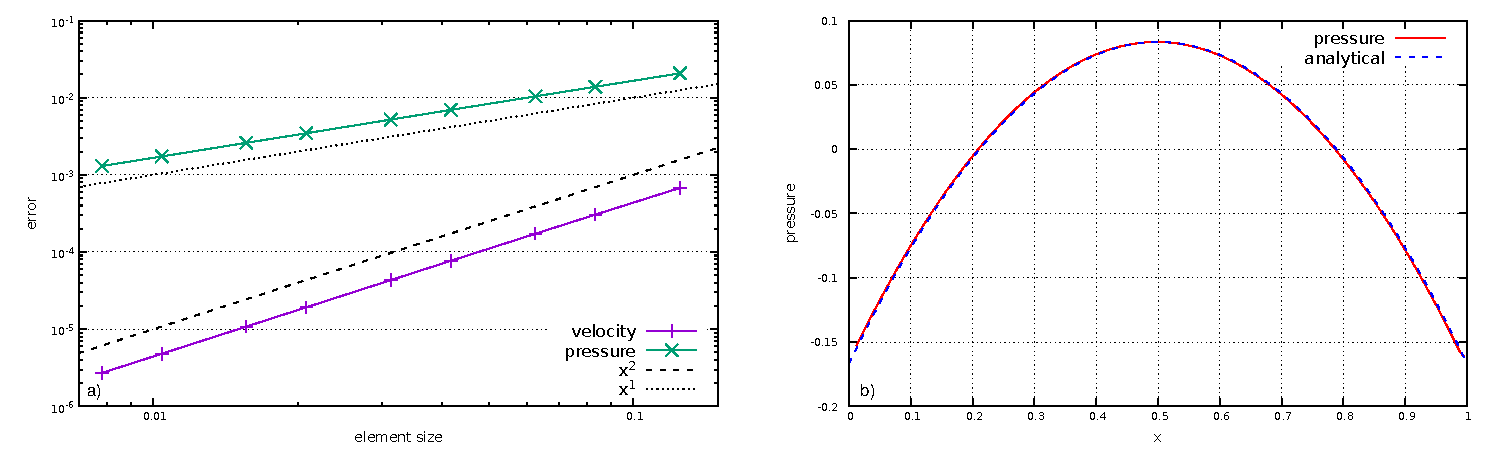
\includegraphics[width=\textwidth]{./Figures/errors.pdf}
\caption{Velocity and pressure error for the Stokes flow experiment between generated and analytical solution as a function of element size (panel a),
and comparison between smoothed pressure and analytical solution as function of $x$ coordinate for a grid resolution of \num{128x128} elements (panel b).}
\label{fig:errors}
\end{figure}

\begin{figure}
\noindent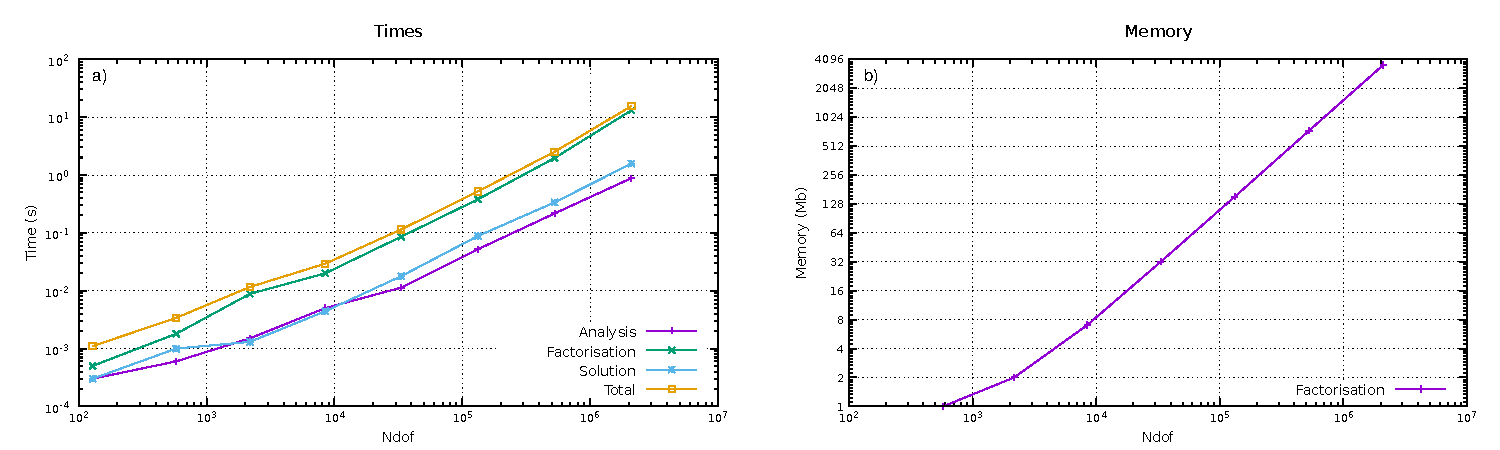
\includegraphics[width=\textwidth]{./Figures/MUMPS.pdf}
\caption{Panel a) Analysis, factorisation, solution and total solve times (panel a) and factorisation memory usage (panel b) as a function of the total number
of degrees of freedom for the Stokes flow experiment.}
\label{fig:MUMPS}
\end{figure}

\subsection{Markers advection}\label{sec:runge}
The 2nd-order Runge-Kutta advection scheme in space is tested by means of the Zalesak disk test \citep{Zalesak1979,Thieulot2014}. The benchmark is performed
in a unit square domain with a grid resolution of \num{32x32} elements and 1000000 markers and values of Courant number between 0.25 and 1.
At $t=0$, the disk is centred at position $(0.5;0.75)$ with a radius $R=0.15$ and has a vertical fissure 0.05 wide and 0.2 high (orange in Fig. \ref{fig:runge})
and with the velocity field prescribed in the entire domain as
\begin{eqnarray}
u(x,y)&=&2\pi\left(y-\frac{L_x}{2}\right)\nonumber \\
v(x,y)&=&-2\pi\left(x-\frac{L_x}{2}\right)\nonumber
\end{eqnarray}
the markers are back to their initial location after a $2\pi$ rotation ($t=1$). The clockwise rotation of the disk at $t=0.25$, 0.5 and 0.75 
is shown in Fig. \ref{fig:runge} (red, blue and green, respectively). The distance from the centre of 1 marker is calculated throughout the rotation to
evaluate the error for different values of Courant number. As expected, the error increase with the increasing of the time step, as shown in 
Fig. \ref{fig:runge_err}. 
All data can be found at \url{https://github.com/aleregorda/Benchmarks/tree/main/Advection/Zalesak_Disk}.

\begin{figure}
\centering
\noindent\includegraphics[width=200px]{./Figures/Zalesak.pdf}
\caption{Position of the Zalesak disk at $t=0$, 0.25, 0.5 and 0.75 (orange, red, blue and green, respectively) for the case with Courant number of 1.}
\label{fig:runge}
\end{figure}

\begin{figure}
\centering
\noindent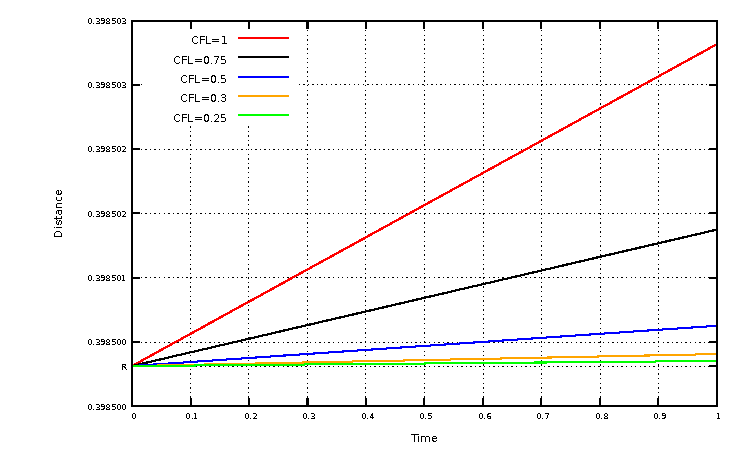
\includegraphics[width=400px]{./Figures/zal_marker.pdf}
\caption{Distance from the centre as function of time for values of Courant number of  of 0.25, 0.3, 0.5, 0.75 and 1 (green, orange, blue, black and red,
respectively). R indicates the distance from the centre considering a perfect circle trajectory.}
\label{fig:runge_err}
\end{figure}

\subsection{Conservative Velocity Interpolation (CVI)}\label{sec:CVI}
The CVI correction is checked by means of the Stokes flow experiment by \citet{Donea2003}, as presented in \ref{sec:stokes}. The advection of Lagrangian
markers is performed using either a 2nd-order or a 4th-order Runge-Kutta scheme with CFL=0.5 and an initial random distribution of 25 markers per element.
Fig. \ref{fig:CVI} shows the minimum and maximum values of markers per element throughout the experiment with and without the CVI correction and using
different Runge-Kutta schemes. The introduction of the CVI correction allows the
tests to run for times longer than $t=2000$ without show empty elements, while tests without the CVI correction stop at approximately $t=600$, when at least
one element goes empty. Fig. \ref{fig:CVI_time} shows the different number of markers per element and the markers distribution at $t=600$ obtained without and
with the CVI correction (panels b and c, respectively) in case of a 2nd-order Runge-Kutta scheme. All data can be found at
\url{https://github.com/aleregorda/Benchmarks/tree/main/Advection/CVI}.
\begin{figure}
\centering
\noindent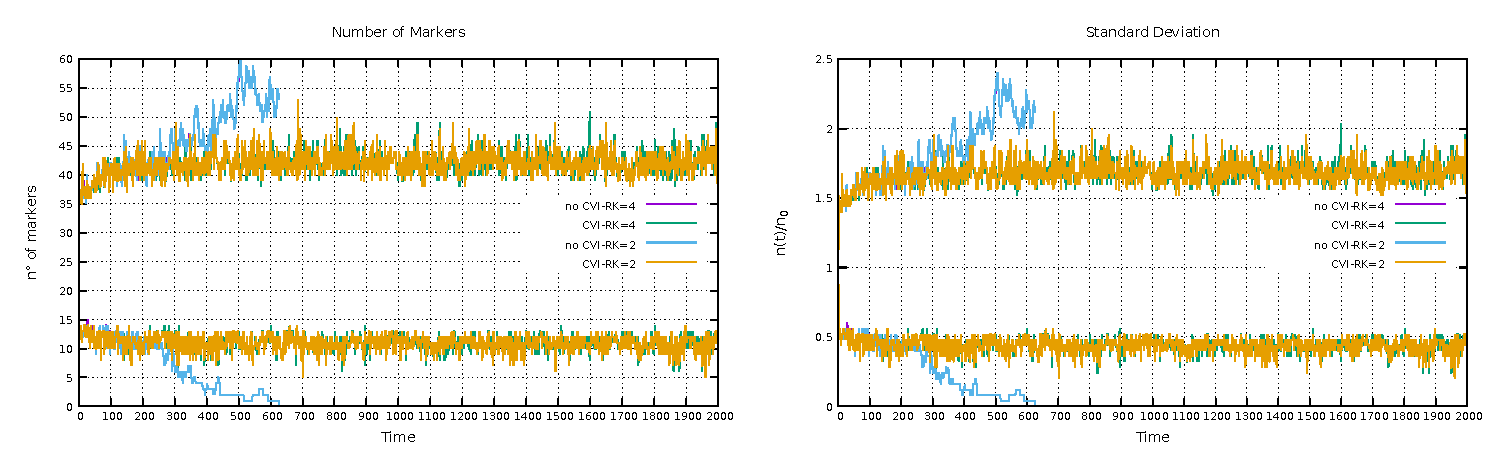
\includegraphics[width=\textwidth]{./Figures/CVI.pdf}
\caption{Maximum and minimum number of markers per element throughout the experiment, with (green and orange lines) or without (purple and blue lines)
the CVI correction and using either a 2nd-order (blue and orange lines) or a 4th-order (purple and green lines) Runge-Kutta scheme.}
\label{fig:CVI}
\end{figure}
\begin{figure}
\centering
\noindent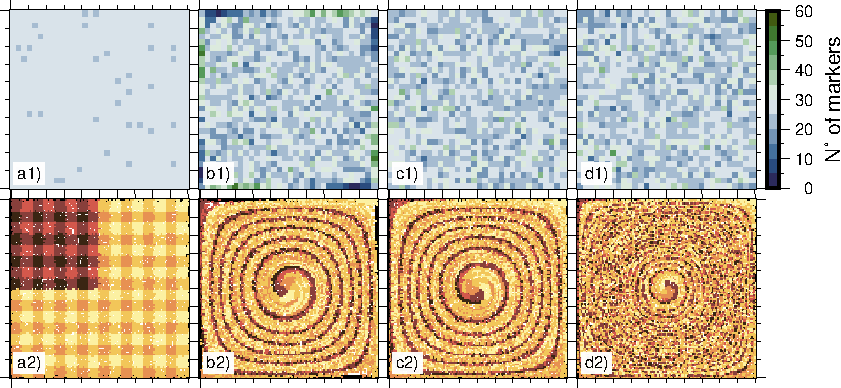
\includegraphics[width=\textwidth]{./Figures/CVI_time.pdf}
\caption{Number of markers per element and markers distribution through time using 2nd.order Runge-Kutta scheme.
Panels a: number of markers per element (panel a1) and distribution of the markers (panel a2) after the first
iteration; panels b and c: comparison between number of markers per element (panels b1 and c1) and markers distribution (panels b2 and c2) without and with
the CVI correction at $t=600$; panels d: number of markers per element (panel d1) and markers distribution (panel d2) in case of CVI correction at $t=2000$.}
\label{fig:CVI_time}
\end{figure}

\subsection{Poiseuille flow}\label{sec:poiseuille}
The domain is a rectangle with $L_x=2$ and $L_y=1$ and constant density and viscosity ($\rho=1$ and $\eta=1$), gravity acceleration $\bm{g}=\bm{0}$ and penalty
parameter $\lambda=10^8$. The grid is composed by \num{40x20} elements. Velocity boundary conditions are set to no slip $(\bm{v}=\bm{0})$ at the top and the
bottom, and a parabolic profile is imposed on the sides, with $u=y(1-y)$ and $v=0$. The analytical solution is then given by:
\begin{eqnarray}
u(x,y)&=&y(1-y)\nonumber \\
v(x,y,)&=&0\nonumber \\
p(x,y)&=&2\eta\left(\frac{L_x}{2}-x\right)\nonumber
\end{eqnarray}

The velocity field predicted by the model follows the expected parabolic profile (Fig. \ref{fig:poiseuille}a and Fig. \ref{fig:poi_plot}a) and, in case of the
classic penalty method with no iterations, the pressure is clearly related to the divergence by means of the penalty parameter (Fig. \ref{fig:poiseuille}b and
c and Fig. \ref{fig:poi_plot}b). Fig. \ref{fig:poiseuille}d shows that one Uzawa iteration is sufficient to bring the divergence down to \num{e-15}, with no
correlation with the pressure field. All data can be found at \url{https://github.com/aleregorda/Benchmarks/tree/main/Momentum_equation/Poiseuille%20Flow}.

\begin{figure}
\noindent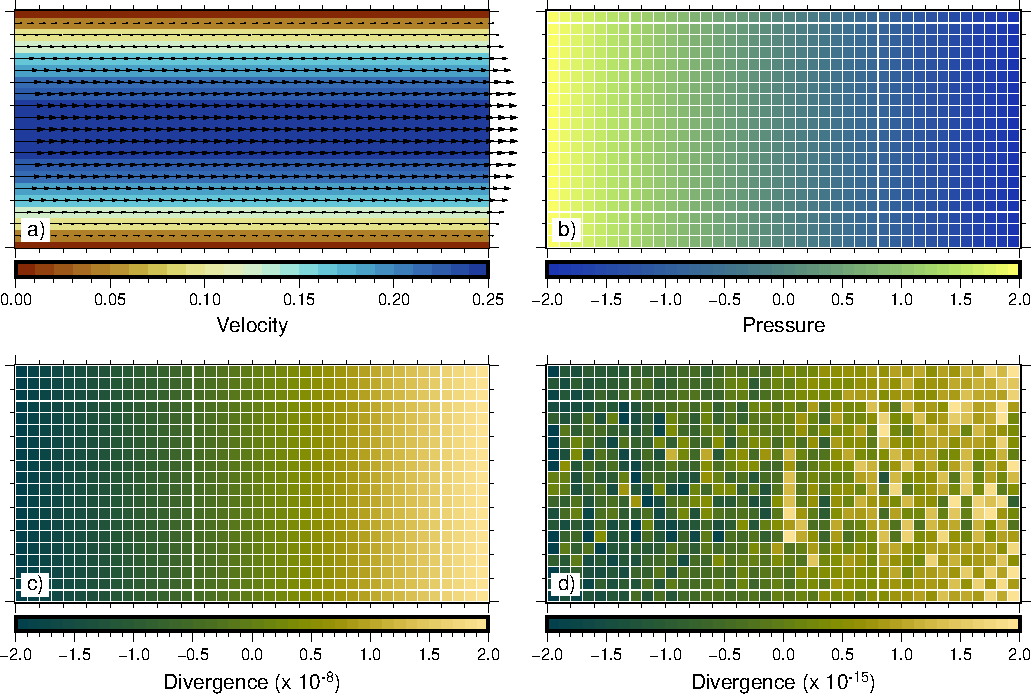
\includegraphics[width=\textwidth]{./Figures/Poiseuille.pdf}
\caption{Velocity field (panel a), pressure (panel b) and divergence velocity of a Poiseuille flow in case of the classic penalty method (no iterations) and
after one Uzawa iteration (panel c and d, respectively).}
\label{fig:poiseuille}
\end{figure}

\begin{figure}
\noindent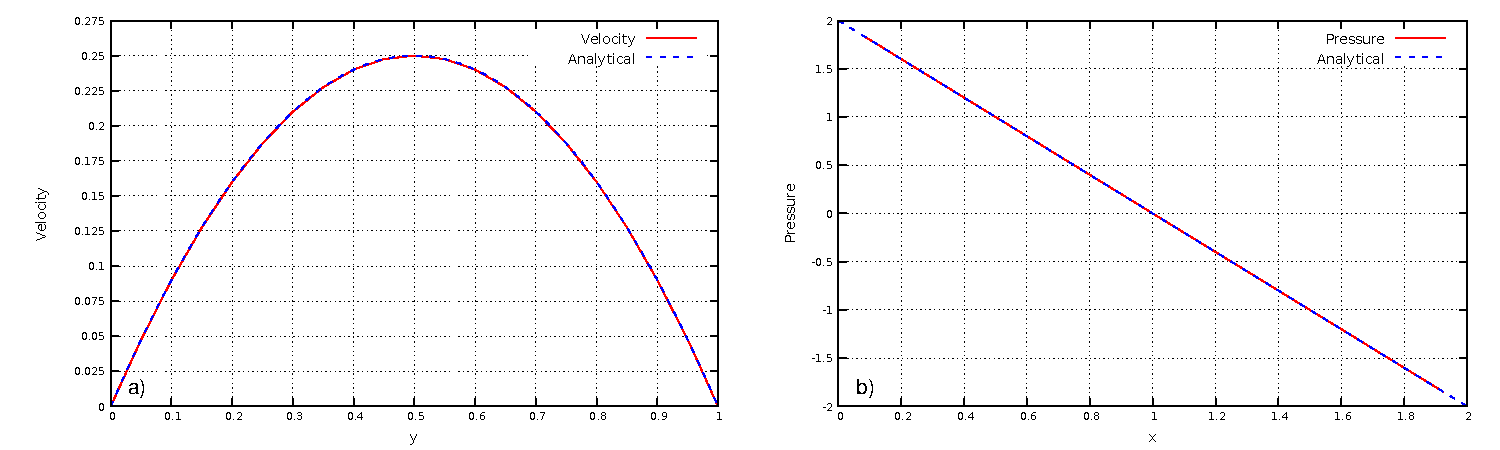
\includegraphics[width=\textwidth]{./Figures/Analytical.pdf}
\caption{Velocity (panel a) and pressure (panel b) field predicted by the model for a Poiseuille flow with respect with their analytical solutions. The
velocity field is plotted as function of the vertical coordinate in $L_x/2$ and the pressure is plotted as function of the x coordinate in $L_y/2$.}
\label{fig:poi_plot}
\end{figure}

\subsection{Instantaneous 2D sphere}\label{sec:ist_sphere}
The domain is a unit square with gravity $\bm{g}=(0,-1)$. The fluid has constant density and viscosity ($\rho_f=1$ and $\eta_f=1$). The sphere is in the middle
of the domain with a radius R = 0.123456798 and has constant density and viscosity ($\rho_s=10^{-2}+\rho_f$ and $\eta_s=10^3 \cdot \eta_f$).
We distinguish three different types of velocity boundary conditions:
\begin{enumerate}
\item FS: free slip conditions on all sides.
\item NS: no slip conditions on all sides.
\item OT: free slip conditions on the sides and the bottom, and open boundary at the top.
\end{enumerate}
All three cases are performed for different grid resolutions, between \num{16x16} and \num{512x512} elements with 50 randomly distributed markers per element,
and different average schemes for the viscosity (harmonic, geometric and arithmetic). The velocity in the centre of the sphere $\bm{v}(0.5;0.5)$), minimum and
maximum velocities ($u_{min}$, $u_{max}$, $v_{min}$, $v_{max}$) and pressures ($p_{min}$, $p_{max}$) on the entire domain, $v_{\textrm{rms}}$ and average pressure on the
entire domain ($p_{avg}$) are compared with solutions generated by ASPECT \citep{KHB12,heister_aspect_methods2,aspect-doi-v2.2.0,aspectmanual} and all results
can be found at \url{https://github.com/cedrict/fieldstone/tree/master/images/stokes_sphere2D} and 
\url{https://github.com/aleregorda/Benchmarks/tree/main/Momentum_equation/Instantaneous_2D_Sphere}. Results in terms of the $v_{\textrm{rms}}$ for NS model 
are also shown in Fig. \ref{fig:inst_sphere}.

\begin{figure}
\centering
\noindent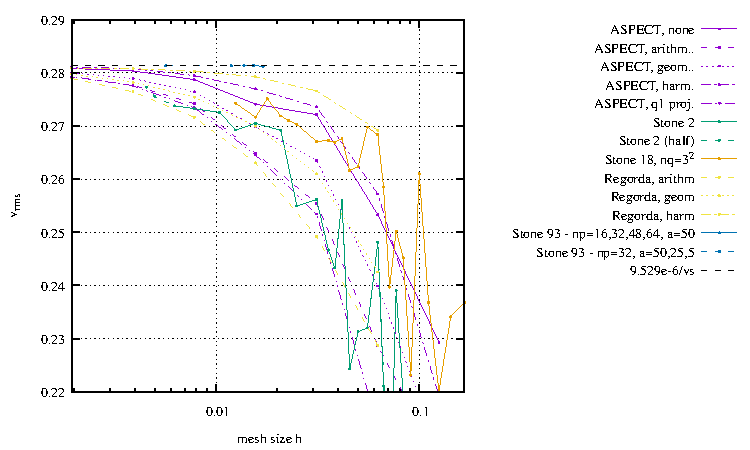
\includegraphics[width=400px]{./Figures/vrms_NS.pdf}
\caption{$v_{\textrm{rms}}$ as function of element size for the instantaneous 2D sphere experiment in case of no slip boundary conditions and with different average
schemes for the viscosity. Results are compared with results obtained by other numerical codes.}
\label{fig:inst_sphere}
\end{figure}

\subsection{Rayleigh-Taylor instability}\label{sec:rayleigh}
This problem has been originally presented by \citet{vanKeken1997} and here it is performed as the isoviscous case (Case 1a). The domain has $L_x=0.9142$ and
$L_y=1$ and gravity $\bm{g}=(0,-1)$. Two fluids with same constant viscosities ($\eta_1=\eta_2=1$) and different densities ($\rho_1=1000$ and $\rho_2=1010$),
with the lighter fluid at the bottom. The initial interface between the fluids is given by $y(x)=0.2+0.02 \cos \left(\frac{\pi x}{L_x}\right)$. The experiment
is performed with different grid sizes (\num{50x50}, \num{80x80}, \num{100x100} and \num{256x256}). A total of 1960000 markers are randomly distributed at the
beginning of the simulation. Velocity boundary conditions are set to no slip at the top and the bottom, and to free slip at the sides of the domain.

$v_{\textrm{rms}}$ as function of time is reported in Fig. \ref{fig:RT}, matching well with results shown by \citet{vanKeken1997}, \citet{Tackley2003} and
\citet{Thieulot2014}. Fig. \ref{fig:rayleigh} shows the evolution of the experiment at different time steps. All data can be found at 
\url{https://github.com/aleregorda/Benchmarks/tree/main/Momentum_equation/Rayleigh_Taylor_experiment/ISOVISCOUS}.

\begin{figure}
\centering
\noindent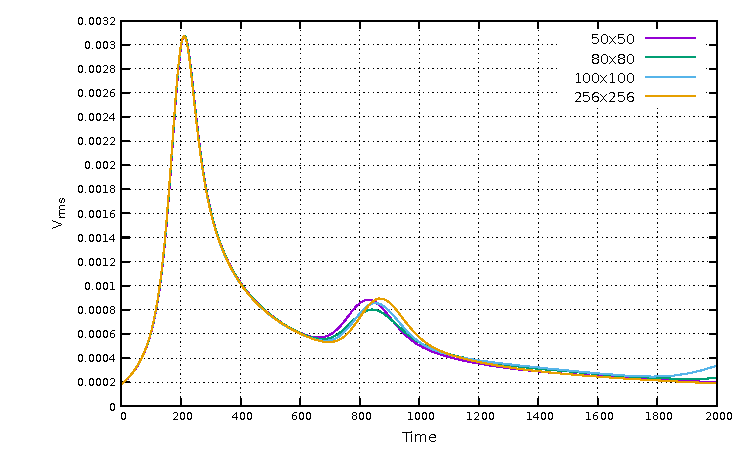
\includegraphics[width=400px]{./Figures/RT.pdf}
\caption{$v_{\textrm{rms}}$ of the Rayleigh-Taylor experiment as function of time for different resolution of the grid.}
\label{fig:RT}
\end{figure}

\begin{figure}
\centering
\noindent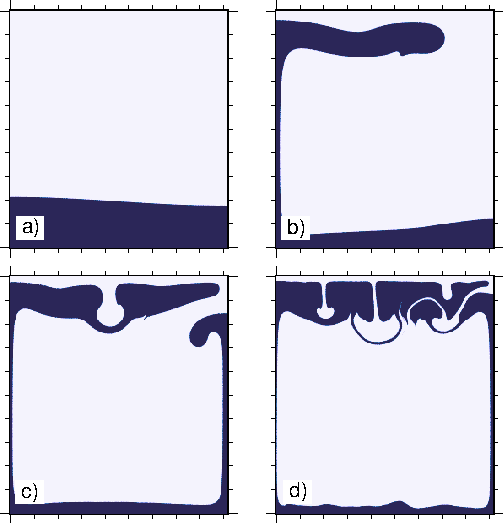
\includegraphics[width=300px]{./Figures/Rayleigh.pdf}
\caption{Evolution of the Rayleigh-Taylor experiment for a grid of \num{256x256} elements at $t=0, 500, 1000$ and $2000$ (panels a, b, c and d, respectively).}
\label{fig:rayleigh}
\end{figure}

\subsection{Falling blocks}\label{sec:block}
This benchmark is described as proposed by \citet{Gerya2003a}, \citet{Gerya2010b} and \citet{Thieulot2011}. The domain is square with $L_x=L_y=$ \SI{500}{\km}
and the grid is composed by \num{50x50} elements with 25 markers in each element. The block is initially centred at ($x=$ \SI{250}{\km}; $y=$ \SI{400}{\km})
and has a size of \num{100x100} km (Fig. \ref{fig:block}a). The fluid surrounding the block has $\eta_f=$ \SI{e21}{\pascal\per\s} and $\rho_f=$
\SI{3200}{\kg\per\cubic\m}. The benchmark tests with different viscosities of the block, with $\eta_b$ from \SIrange{e15}{e27}{\pascal\per\s}. In each
experiment also the density $\rho_b$ of the block varies from \SIrange{3220}{9900}{\kg\per\cubic\m}. Velocity boundary conditions are set to free slip
conditions on all sides of the domain. Density distributions at $t=$ \SI{20}{\mega\year} for $\rho_b=$ \SI{3300}{\kg\per\cubic\m} and different $\eta_b$
are plotted in Fig. \ref{fig:block}b-f, showing that the code correctly preserve the block geometry in case of large viscosity contrast, with a block stiffer
than the surrounding fluid (Fig. \ref{fig:block}f).

The velocity in the centre of the falling block at $t=0$ is measured for all experiments and, since the velocity should increase with density contrast, the
quantity $\bm{v}/(\rho_b-\rho_f)$ is plotted as function of the viscosity contrast. All results perfectly match with those from \citet{Gerya2010b} and they
line up on a single curve, demonstrating that the code can correctly deal with large viscosity and density contrasts (Fig. \ref{fig:falling}). All data can be 
found at \url{https://github.com/aleregorda/Benchmarks/tree/main/Momentum_equation/Falling%20blocks}.

\begin{figure}
\noindent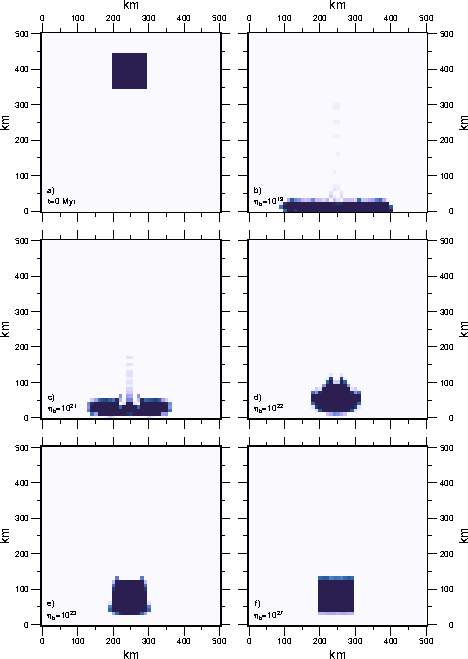
\includegraphics[width=300px]{./Figures/Block.pdf}
\centering
\caption{Density evolution of the falling block experiment at $t=$ \SI{0}{\mega\year} (panel a) and $t=$ \SI{20}{\mega\year} for different viscosities of the
block (panels b-f).}
\label{fig:block}
\end{figure}

\begin{figure}
\centering
\noindent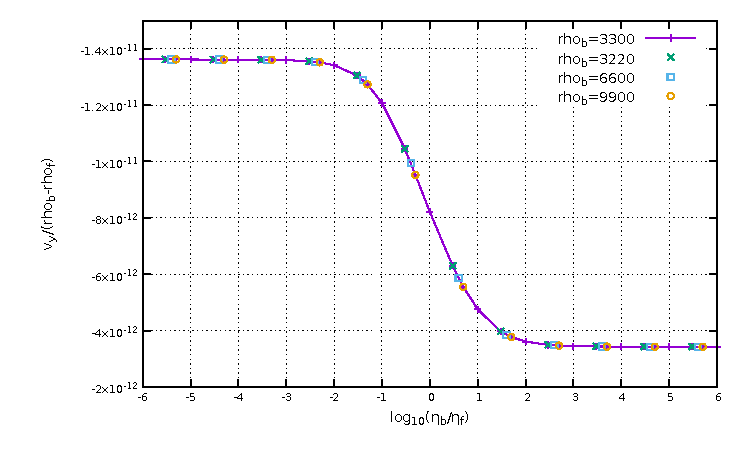
\includegraphics[width=400px]{./Figures/Falling.pdf}
\caption{Initial velocity relative to the density contrast at the centre of the falling block as function of the viscosity contrast between the block and the
surrounding fluid.}
\label{fig:falling}
\end{figure}

\subsection{2D time-dependent Stokes sphere with deformable free surface}\label{sec:sphere}
This experiment is performed in a unit square domain with the gravity acceleration fixed to $g_y=-1$. The sphere has $\rho_s=2$ and $\eta_s=10^3$ and is
initially centred at ($0.5;0.6$) with radius $R=0.123456789$. The fluid surrounding the sphere has $\rho_f=1$ and $\eta_f=1$ and occupies the domain for
$y\leq 0.75$, while for $y>0.75$ the air has $\rho_a=0$ and $\eta_a=10^{-3}$. Velocity boundary conditions are set to free slip on all sides. The Courant
number is set to 0.25. The experiments run for 200 s using grid resolutions from \num{150x150} to \num{512x512} elements, with 25 randomly distributed markers
per element, and for different average schemes for the viscosity. The interface between the fluid and the air is tracked by means of the markers chain. Results
in terms of velocity and pressure fields and topography variations are compared with results obtained with ASPECT
\citep{KHB12,heister_aspect_methods2,aspect-doi-v2.2.0,aspectmanual} and they can be found at
\url{https://github.com/cedrict/fieldstone/tree/master/images/stokes_sphere_fs2D} and
\url{https://github.com/aleregorda/Benchmarks/tree/main/Surface_processes/Time_dependent_sphere}. Results in terms of the $v_{\textrm{rms}}$ in case of 
an arithmetic average are also shown in Fig. \ref{fig:inst_spherefs}.

\begin{figure}
\centering
\noindent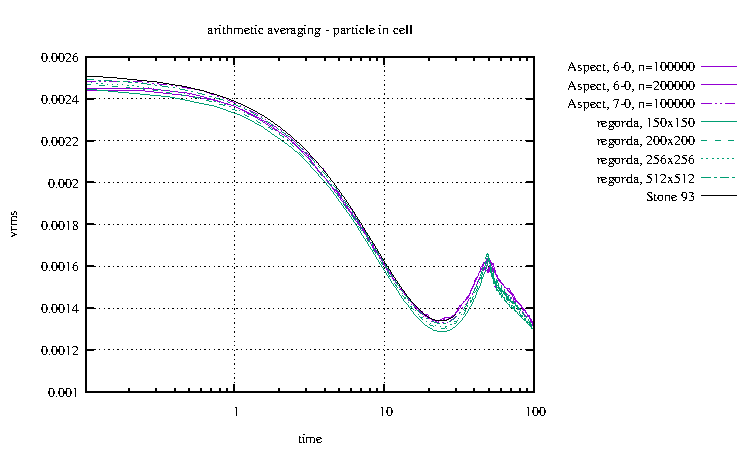
\includegraphics[width=400px]{./Figures/vrms_arithm.pdf}
\caption{$v_{\textrm{rms}}$ for different grid resolutions as function of time for the 2D time-dependent Stokes sphere experiment in case of an arithmetic average.
Results are compared with results obtained by ASPECT.}
\label{fig:inst_spherefs}
\end{figure}

\subsection{Free surface stabilisation}\label{sec:stab}
The benchmark is performed as discussed in \citet{Kaus2010a} and \citet{Thieulot2014}. The domain is square with $L_x=L_y=$ \SI{500}{\km} and a grid resolution
of \num{200x200} elements, each of them containing 16 markers. A buoyant fluid with $\rho_1=$ \SI{3200}{\kg\per\cubic\metre} and $\eta_1=$ \SI{e20}{\pascal\s}
is overlain by a denser fluid with $\rho_2=$ \SI{3300}{\kg\per\cubic\metre} and $\eta_2=$ \SI{e21}{\pascal\s}. The initial interface between the fluids has an
initial sinusoidal shape of 5 km amplitude. Velocity boundary conditions are set to free slip conditions at the sides and no slip at the bottom, while the top
is free surface. The experiment is performed with various fixed time steps, without the use of the Courant number. The vertical position of the free surface at
$x=L_x$ is tracked for each simulation, with or without the stabilisation algorithm.

The results show an instability (drunken sailor effect) increasing the time step in case that the stabilisation algorithm is not activated
($dt=$ \SI{4200}{\year}, green line in Fig. \ref{fig:stab}), as already observed by \citet{Kaus2010a} and \citet{Thieulot2014}. Activating the algorithm the
instability is fixed and the simulation remains stable using time step up to \SI{50000}{\year} (red line in Fig. \ref{fig:stab}). All data can be 
found at \url{https://github.com/aleregorda/Benchmarks/tree/main/Surface_processes/Stabilisation_algorithm}.

\begin{figure}
\centering
\noindent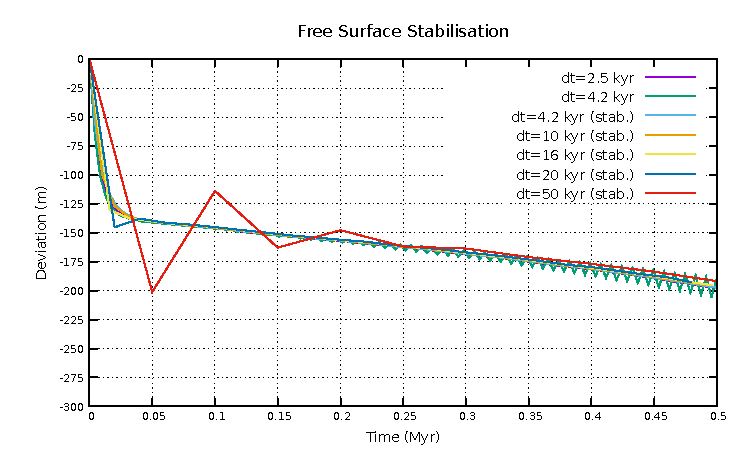
\includegraphics[width=400px]{./Figures/Kaus_random.pdf}
\caption{Evolution of the y coordinate in $x=L_x$ as function of time for different time steps, with and without the stabilisation algorithm.}
\label{fig:stab}
\end{figure}

\subsection{Topography relaxation}\label{sec:crameri}
This experiment is performed as in \citet{Crameri2012} using free surface and sticky air (Case 1). The domain is rectangular with $L_x=$ \SI{2800}{\km} and
$L_y=$ \SI{700}{\km} in case of free surface and $L_y=$ \SI{800}{\km} in case of sticky air ($h_{st}=$ \SI{100}{\km}). The grid is composed by \num{256x64}
elements for the free surface \num{560x320} elements for the sticky air. For both cases, there is a mantle of 600 km thickness with $\eta_m=$ \SI{e21}{\pascal\s}
overlain by a highly viscous cosine-shaped lithosphere with thickness between 93 and 107 km and $\eta_l=$ \SI{e23}{\pascal\s}. Both mediums have $\rho=$
\SI{3300}{\kg\per\cubic\metre}. In case of sticky air experiment, the air has $\rho_a=$ \SI{0}{\kg\per\cubic\metre} and $\eta_a=$ \SI{e18}{\pascal\s}. The
gravity acceleration is set to $g_y=$ \SI{-10}{\metre\per\square\s}. Velocity boundary conditions are set to no slip at the bottom and free slip at the sides
of the domain. In case of sticky air, velocities on top are set to free slip conditions.

The maximum topography as function of time ($h(t)$) can be analytically derived in according to \[h(t)=h_0 \exp(\gamma t)\]
where $h_0=7$ km is the initial topography, $\gamma=\num{-0.2139e-11}$ is the characteristic relaxation rate and $t$ is the time (black line in Fig.
\ref{fig:crameri}). Maximum topography at the characteristic relaxation time $t_{rlx}=$ \SI{14.825}{\kilo\year} can be found to be $h_{rlx}=$ \SI{2576}{\m}.
The results show that a viscosity of the air of \SI{e18}{\pascal\s} is needed in case of $h_{st}=$ \SI{100}{\km} to correctly describe the topography relaxation
for this problem, as pointed out by \citet{Crameri2012} (purple line in Fig. \ref{fig:crameri}). The case with a true free surface well follows the analytical
solution (orange line in Fig. \ref{fig:crameri}). In particular, at the relaxation time in case of the true free surface predicts a maximum topography of
\SI{2570}{\m}, with an error of \SI{6}{\m} with respect to the analytical solution. Results are also compared with results obtained with a free surface in
UNDERWORLD (\num{256x64} elements) and SULEC (\num{401x201} elements) (with courtesy from \citealp{Crameri2012}). All data can be 
found at \url{https://github.com/aleregorda/Benchmarks/tree/main/Surface_processes/Topography_relaxation}.

\begin{figure}
\centering
\noindent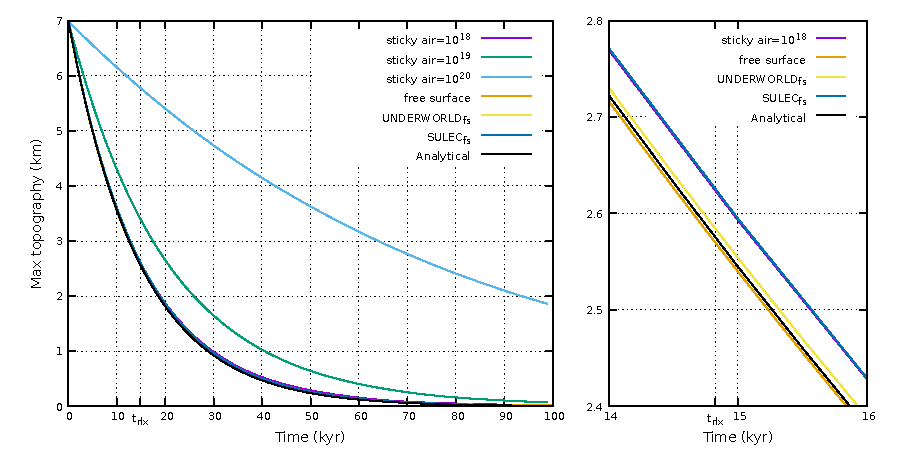
\includegraphics[width=400px]{./Figures/Crameri.pdf}
\caption{Maximum topography as function of time for the Crameri benchmark (coloured lines) in comparison with the analytical solution (black line) and results
obtained with UNDERWORLD (yellow line) and SULEC (blue line).}
\label{fig:crameri}
\end{figure}

\subsection{Spontaneous subduction}\label{sec:subduction}
This experiment is performed as presented by \citet{Schmeling2008}, in case of both a sticky air and a true free surface and using different average schemes
for the viscosities. The domain is rectangular with $L_x=$ \SI{3000}{\km} and $L_y=$ \SI{700}{\km}, a grid resolution of \num{256x64} elements with 50 markers
per element and Courant number of 0.01. At the beginning of the simulation, a 100 km-thick lithospheric layer with $\rho_m=$ \SI{3300}{\kg\per\cubic\metre}
and $\eta_m=$ \SI{e23}{\pascal\s} is located at the top of the domain for $x$ between 1000 and 3000 km, while the asthenospheric mantle has $\rho_m=$
\SI{3200}{\pascal\s} and $\eta_m=$ \SI{e21}{\pascal\s}. In addition, a 200 km-depth lithospheric slab is already subducted in the mantle in order to have
a spontaneous subduction. In case of sticky air, $L_y=750$ km and a 50 km-thick air layer with $\eta_a$ from \SIrange{e19}{e21}{\pascal\s} overlie the mantle.
Velocity boundary conditions are set to free slip on the sides and on the bottom of the domain. In case of sticky air, velocities on the top boundary are set
to free slip conditions as well.

The maximum depth of the slab is tracked for all the simulations (Fig. \ref{fig:subduction}) and they are compared with results obtained by
\citet{Schmeling2008} with models with regular grids and comparable grid resolutions (rectangles in Fig. \ref{fig:subduction}). Low viscous sticky air models
(i.e., \SI{e19}{\pascal\s}) enlighten a strong dependence of the sinking velocity with the chosen average scheme (dashed lines in Fig. \ref{fig:subduction}),
while high viscous sticky air models (i.e., \SI{e21}{\pascal\s}) show a higher resistance at the trench, underestimating the correct solution (dotted lines in
Fig. \ref{fig:subduction}). A high resistance at the trench can be also observed in case of a true free surface for the low resolution grid used (continuous
lines in Fig. \ref{fig:subduction}), as pointed out by \citet{Schmeling2008}. All data can be 
found at \url{https://github.com/aleregorda/Benchmarks/tree/main/Surface_processes/Spontaneous_subduction}.

\begin{figure}
\centering
\noindent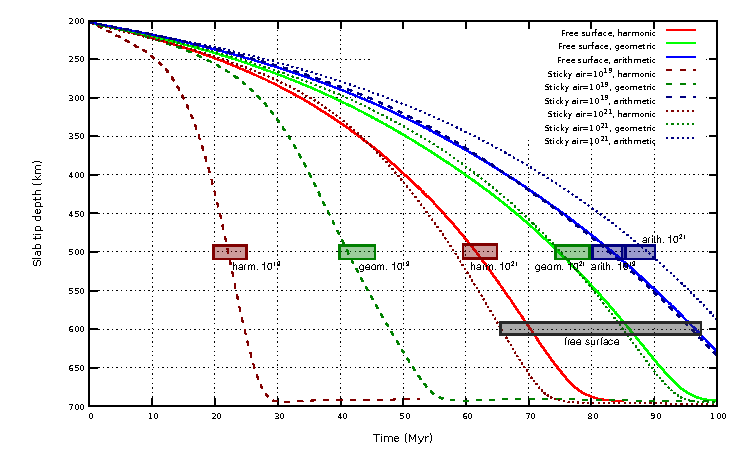
\includegraphics[width=400px]{./Figures/Subduction.pdf}
\caption{Maximum depth of the slab as function of time for all the simulations of the \citet{Schmeling2008} benchmark, in case of harmonic, geometric and
arithmetic means (red, green and blue lines, respectively) using a sticky air or a true free surface (discontinuous and continuous lines, respectively).
Red, green and blue rectangular areas indicate the range of times from \citet{Schmeling2008} when the slab tip reaches \SI{500}{\km} in case of sticky air,
while the grey rectangular area indicates the range of times from \citet{Schmeling2008} when the slab tip reaches \SI{600}{\km} in case of true free surface.}
\label{fig:subduction}
\end{figure}

\subsection{The slab detachment}\label{sec:slab}
The slab detachment benchmark is performed as described by \citet{Schmalholz2011} and \citet{Glerum2018}. The domain is rectangular with $L_x=$ \SI{1000}{\km}
and $L_y=$ \SI{660}{\km} and a grid resolution of \num{256x256} elements. A non-linear viscous T-shaped layer with $\rho_l=$ \SI{3300}{\kg\per\cubic\metre} is
placed at the top of the domain and surrounded by a linear viscous fluid with $\rho_f=$ \SI{3150}{\kg\per\cubic\m}. The top layer is 80 km-thick and a 250
km-long and 80 km-wide slab is placed at $x=L_x/2$ (Fig. \ref{fig:slab}a). The effective viscosity of the top layer is given by
\[\eta_{eff}=\eta_0 I_2^{\frac{(1-n)}{n}}\]
with $\eta_0=$ \SI{4.75e11}{\pascal\s} and $n=4$, while the surrounding fluid has $\eta_f=$ \SI{e21}{\pascal\s}. The effective viscosity is capped between
$\eta_{min}=$ \SI{e21}{\pascal\s} and $\eta_{max}=$ \SI{e25}{\pascal\s}. Velocity boundary conditions are set to free slip at the top and the bottom, and to
no slip at the sides of the domain.

The sinking of the slab determines a decrease of the effective viscosity in the T-shaped layer during the first part of the evolution (Fig. \ref{fig:slab}a),
as consequence of local strain rates, while effective viscosities increase up to $\eta_{max}$ in the top layer after approximately \SI{20}{\mega\year}, when
necking is complete (Fig. \ref{fig:slab}b).

The width of necking is tracked by means of markers position at the side of the slab. Necking width and time are normalised in function of the initial slab
(\SI{80}{\km}) and the characteristic time ($t_c=$ \SI{7.1158e14}{\s}) \citep{Schmalholz2011,Glerum2018}. The results in case of arithmetic, geometric and
harmonic mean of the viscosity are shown in Fig. \ref{fig:necking}, compared with results from \citet{Glerum2018} for which an infinity norm mean was used.
The influence of the average schemes agrees with results shown in Section \ref{sec:subduction}. All data can be 
found at \url{https://github.com/aleregorda/Benchmarks/tree/main/Nonlinear_visco_plasticity/Slab_detachment}.

\begin{figure}
\noindent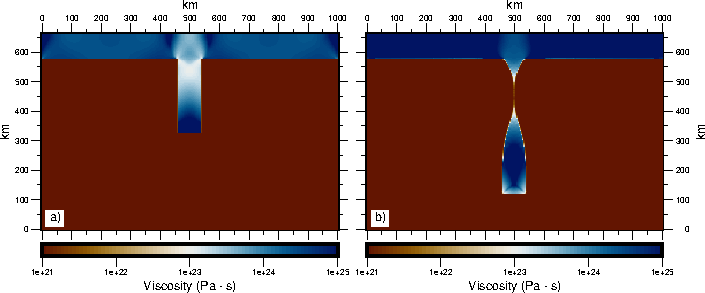
\includegraphics[width=\textwidth]{./Figures/Slab.pdf}
\caption{Effective viscosity for the slab detachment benchmark at the beginning of the evolution (panel a) and when necking is complete (panel b).}
\label{fig:slab}
\end{figure}

\begin{figure}
\centering
\noindent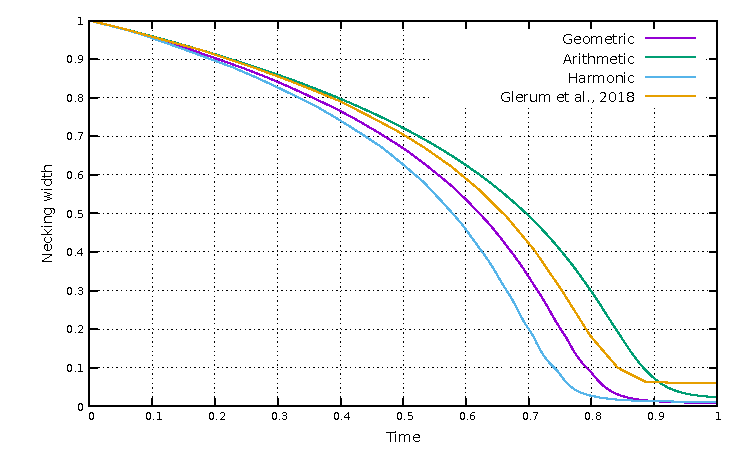
\includegraphics[width=400px]{./Figures/Necking.pdf}
\caption{Normalised width of the necking of the slab detachment benchmark as function of normalised time.}
\label{fig:necking}
\end{figure}

\subsection{The indenter experiment}\label{sec:indenter}
The indenter benchmark simulate a rigid punch on a purely plastic von Mises material, for which exists an analytical solution
\citep{Thieulot2008,Thieulot2014,Glerum2018}. The domain is a unit square with a grid resolution of \num{256x256} elements. The gravity acceleration is set
to $\bm{g}=\bm{0}$ and effective viscosity is capped using $\eta_{min}=10^{-4}$ and $\eta_{max}=10^3$. The tolerance for the convergence of the non-linear
solution is $tol=10^{-9}$, with a maximum number of non-linear iterations set to 500. The medium in the domain has $\rho=0.01$, an initial viscosity
$\eta_0=10$, cohesion $C=1$ and an angle of internal friction $\phi=0$°. Velocity boundary conditions are set to no slip at the bottom and free slip at the
sides of the domain. The top of the domain is open with the exception of the central portion (punch area) with width $w_p=0.125$, where $v=-1.05$ and $u$ is
fixed either to 0 (rough punch experiment) or free (smooth punch experiment).

Fig. \ref{fig:indenter} show the results in terms of viscosity (panels a and b), strain rate (panels c and d), velocity (panels e and f) and pressure
(panels g and h) for both experiments. The analytical solution indicate that pressure at ($0.5;1$) and ($0.5 \pm w_p;1$)is $p=\pi +1$ and $p=1$, respectively
(black and red lines in Fig. \ref{fig:smooth_p}). Fig. \ref{fig:smooth_p} shows a clear improvement in the pressure solution when passing from a rough to a
smooth punch (green and blue lines in Fig. \ref{fig:smooth_p}, respectively), as previously observed by \citet{Thieulot2014} and \citet{Glerum2018}. 
All data can be found at \url{https://github.com/aleregorda/Benchmarks/tree/main/Nonlinear_visco_plasticity/Indenter}.

\begin{figure}
\centering
\noindent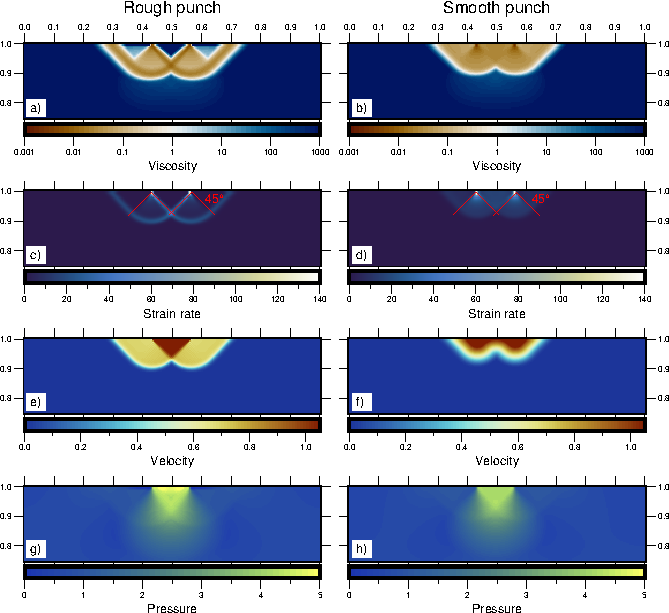
\includegraphics[width=400px]{./Figures/Indenter.pdf}
\caption{Viscosity (panels a and b), strain rate (panels c and d), velocity (panels e and f) and pressure (panels g and h) fields for rough (left column) and
smooth (right column) punch experiments.}
\label{fig:indenter}
\end{figure}

\begin{figure}
\centering
\noindent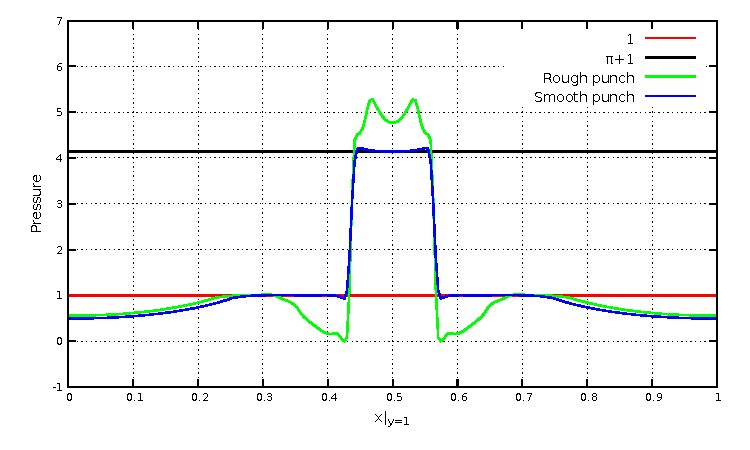
\includegraphics[width=400px]{./Figures/Smooth_Rough.pdf}
\caption{Nodal pressure in function of the x coordinate at $y=1$ for rough (green line) and smooth (blue line) punch experiment. Black and red lines indicate
the analytical solution at $x=0.5$ and $x=0.5 \pm w_p$, respectively.}
\label{fig:smooth_p}
\end{figure}

\subsection{The brick experiment}\label{sec:brick}
An instantaneous version of the brick benchmark is performed to verify the correctness of the pressure-dependent plasticity for different angle of internal
friction, as proposed by \citet{Glerum2018}. The domain is rectangular with $L_x=$ \SI{40}{\km} and $L_y=$ \SI{10}{\km} and a grid resolution of \num{512x128}
elements. The gravity acceleration is set to $g_y=$ \SI{-10}{\m\square\s} and effective viscosity is capped using $\eta_{min}=$ \SI{e19}{\pascal\s} and
$\eta_{max}=$ \SI{e26}{\pascal\s}. The tolerance for the convergence of the non-linear solution is $tol=10^{-7}$, with a maximum number of non-linear iterations
set to 1000. A 800 m-wide and 400 m-height inclusion with $\eta_b=$ \SI{e20}{\pascal\s} and $\rho_b=$ \SI{2700}{\kg\per\cubic\m} is placed at the bottom of the
domain at $x=L_x/2$. The inclusion is surrounded by a non-linear viscous medium with $\rho_m=$ \SI{2700}{\kg\per\cubic\m}, an initial viscosity of
\SI{e23}{\pascal\s}, a linear viscous viscosity of \SI{e25}{\pascal\s} and a cohesion of \SI{40}{\mega\pascal}. Velocities are set to free slip conditions at
the bottom of the domain and the top is open. Velocities on sides of the domain are fixed to $u=$ \SI{+-2e-11}{\m\per\s} and $v=0$. The experiment is performed
in compressional and extensional contexts with an angle of internal friction $\phi$ of the non-linear medium variable between 0° and 30°.

As expected, two shear bands stem from the inclusion with variable angles in relation to both the dynamics context and the internal friction angle. Shear band
angles formed at 45° for $\phi=0$° in both extensional and compressional contexts (Fig. \ref{fig:brick_beam}a), while they are different in case of $\phi\neq0$°.
Shear band angles in case of $\phi=20$° are shown for compression and extension in Fig. \ref{fig:brick_beam}b  and c, respectively. Values of shear band angles
as function of internal friction angles from 0° to 30° are extracted at different depths and minimum and maximum values are plotted in Fig. \ref{fig:brick},
in comparison with theoretical Roscoe, Arthur and Coulomb shear band angles. For all tests the tolerance for nonlinear convergence is defined $tol=10^{-7}$
and none converges before the maximum number of iterations ($it_{max}=1000$) is reached. However, tests with internal friction angles up to 15° show a constant
decrease of the velocity residuals, which can not be observed for for tests with higher internal friction angles (Fig. \ref{fig:convergence}). 
All data can be found at \url{https://github.com/aleregorda/Benchmarks/tree/main/Nonlinear_visco_plasticity/Brick_experiment}.

\begin{figure}
\centering
\noindent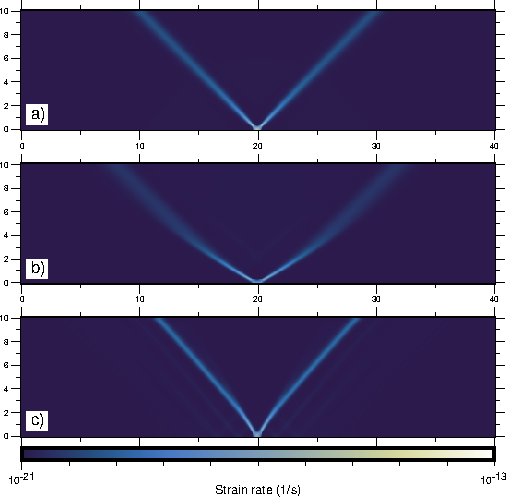
\includegraphics[width=400px]{./Figures/Brick_Beam.pdf}
\caption{Shear band angles predicted for the brick experiment for $\phi=0$° (panel a) and for $\phi=20$° in case of compression and extension (panels b and c,
respectively).}
\label{fig:brick_beam}
\end{figure}

\begin{figure}
\centering
\noindent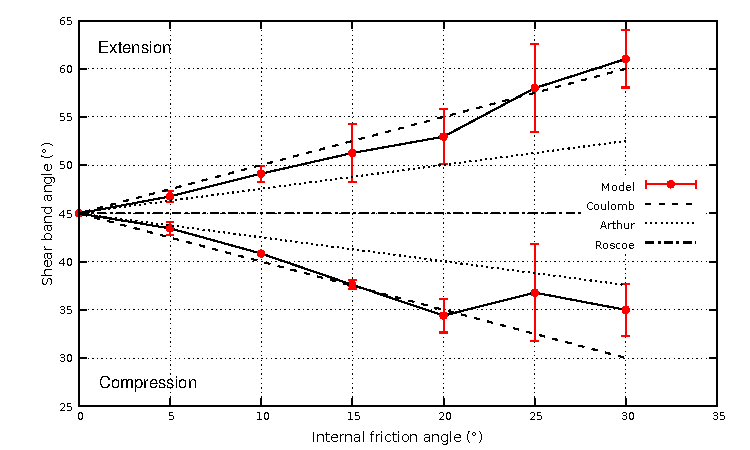
\includegraphics[width=400px]{./Figures/Brick.pdf}
\caption{Shear band angles predicted for the brick experiment in case of compressional and extensional contexts as function of different internal angle of
friction (continuous black line and red dots), compared with theoretical Roscoe, Artur and Coulomb angles (discontinuous black lines). Red lines indicate the
range of angles calculated at different depths.}
\label{fig:brick}
\end{figure}

\begin{figure}
  \centering
  \noindent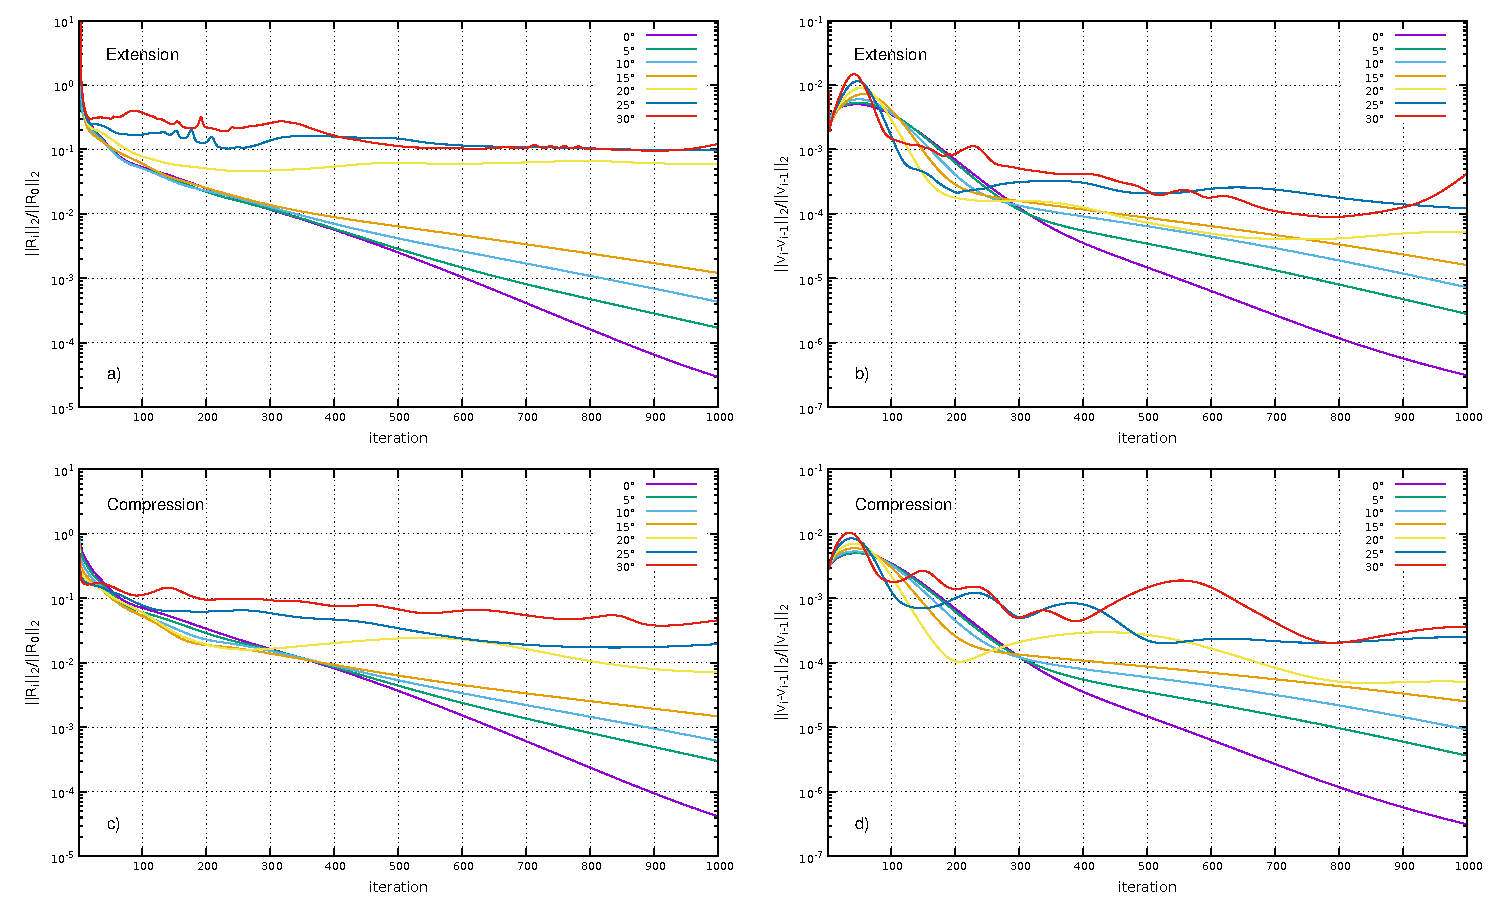
\includegraphics[width=500px]{./Figures/convergence.pdf}
  \caption{Convergence rates for all tests. Normalised residuals (left column) are compared with velocity residuals (right column) for extensional (first row)
  and compressional (second row) settings.}
  \label{fig:convergence}
  \end{figure}

\subsection{Advection stabilisation}\label{sec:advection}
The 1D advection problem proposed by \citet{Donea2003} and \citet{Thieulot2011} is performed to verify the effectiveness of the SUPG method to stabilise the
advection term of the energy equation. The domain is a 1D segment with $L_x=1$ composed by 50 elements and a discontinuity in the thermal field placed at
$x=0.25$. Temperature is set to 1 for $x \leq 0.25$ and to 0 for $x > 0.25$. Velocity is set to ${u}=1$ in the entire domain. The simulation is performed for
250 time steps, with $dt=0.002$, so the thermal discontinuity should be at $x=0.75$ at the end of the simulation.

Temperature profiles at the end of the simulation are shown in \ref{fig:advection} as function of the dimensionless coefficient $\gamma=\tau \bm{v}/h$. In case
of the classic Galerkin method ($\gamma=0$, blue line in \ref{fig:advection}) the final thermal profile is characterised by strong oscillations, which are
eliminated in case of the SUPG method ($\gamma=0.045$, orange line in \ref{fig:advection}). 
All data can be found at \url{https://github.com/aleregorda/Benchmarks/tree/main/Energy_equation/Advection_stabilisation}.

\begin{figure}
\centering
\noindent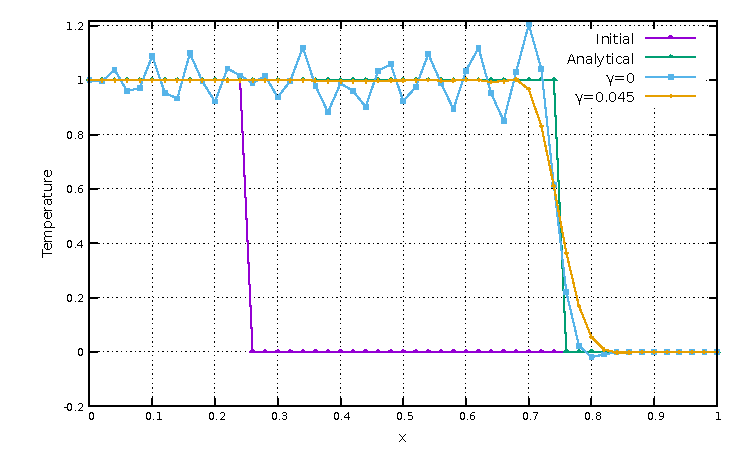
\includegraphics[width=400px]{./Figures/Advection.pdf}
\caption{Temperature profile as function of \textit{x} for the advection stabilisation benchmark. Purple line indicates the initial temperature profile; the
green line indicates the analytical temperature profile after 250 time steps; blue line indicates the temperature profile after 250 time steps in case of the
classic Galerkin method ($\gamma=0$); orange line indicates the temperature profile after 250 time steps in case of the SUPG method ($\gamma=0.045$).}
\label{fig:advection}
\end{figure}

\subsection{Shear heating}\label{sec:simple_shear}
This exercise is performed in an unit square domain composed by \num{128x128} elements. The velocity field is prescribed on the entire domain with
$\bm{v}=(L_y-y)y\bm{e_x}$; viscosity, density and specific heat are fixed to 1, while thermal conductivity and radiogenic energy are fixed to 0. Therefore,
the energy equation (Eq. \ref{eq:energy}) can be simplified as \[\frac{\partial T}{\partial t}=H_s\] and fixing $T(t=0)=0$, the temperature can be find as
\[T(t)=H_s t\]
In this case we have
\begin{eqnarray}
\dot{\epsilon_{xx}}&=&\frac{\partial u}{\partial x}=0 \nonumber \\
\dot{\epsilon_{yy}}&=&\frac{\partial v}{\partial y}=0 \nonumber \\
\dot{\epsilon_{xy}}&=&\frac{1}{2}\left(\frac{\partial v}{\partial x}+\frac{\partial u}{\partial y}\right)=\frac{1}{2}(L_y-2y)\nonumber
\end{eqnarray}
and, simplifying Eq. \ref{eq:shear}, shear heating can be calculated as \[H_s(x,y)=(1-2y)^2\]

The solution predicted by the model in terms of velocity, temperature and shear heating match well with the analytical solutions (Fig. \ref{fig:analytical_en}). 
All data can be found at \url{https://github.com/aleregorda/Benchmarks/tree/main/Energy_equation/Simple_shear}.

%\begin{figure}
%\centering
%\noindent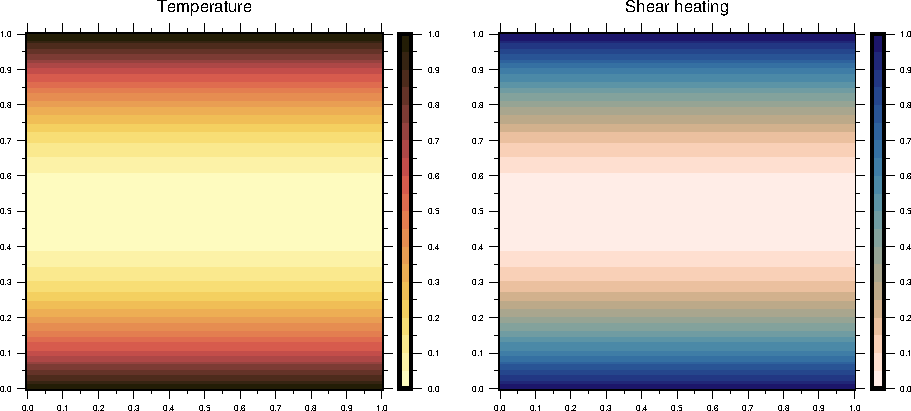
\includegraphics[width=400px]{./Figures/Energy_Thieulot.pdf}
%\caption{Temperature and shear heating predicted by the model after 1 time step.}
%\label{fig:en_thieulot}
%\end{figure}

\begin{figure}
\centering
\noindent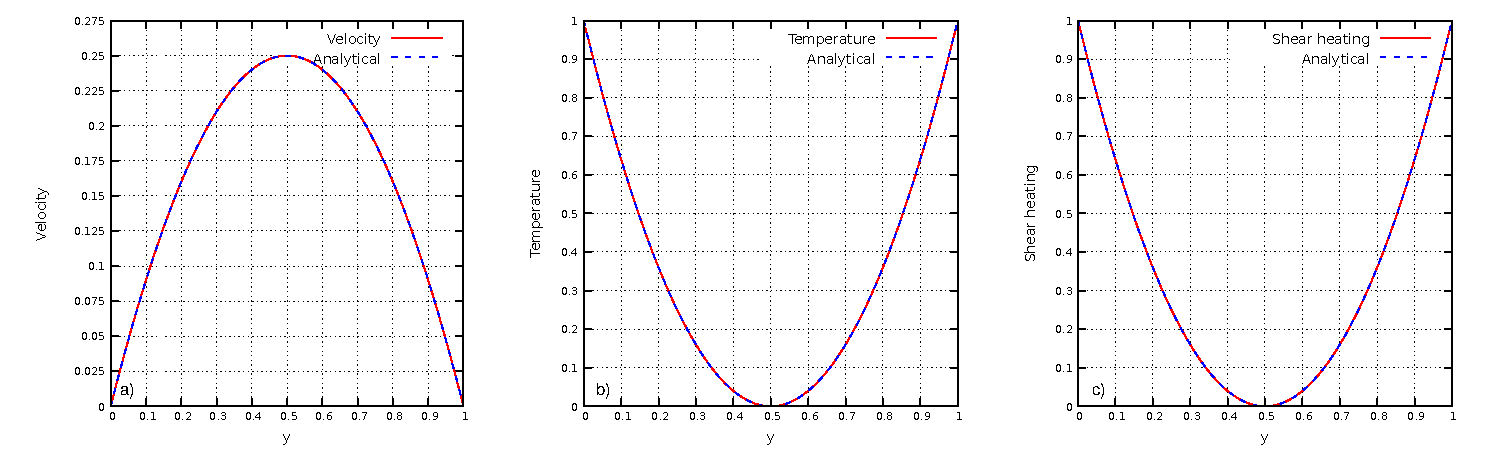
\includegraphics[width=500px]{./Figures/Analytical_Shear.pdf}
\caption{Velocity (panel a), temperature (panel b) and shear heating (panel c) as function of the \textit{y} coordinate for the simple shear experiment. The
solutions predicted by the model (red lines) are compared with the analytical solutions (dashed blue lines).}
\label{fig:analytical_en}
\end{figure}

\subsection{Shear and adiabatic heating}\label{sec:shear}
This problem is performed as presented in Exercise 9.4 in \citet{Gerya2010b}. Two materials are vertically separated in a rectangular domain with $L_x=$
\SI{1000}{\km}, $L_y=$ \SI{1500}{\km} and a grid resolution of \num{30x20} elements. Constant thermal coefficient expansion ($\alpha=$ \SI{3e-5}{\per\kelvin}),
temperature ($T=$ \SI{1300}{\kelvin}) and gravity acceleration ($g_y=$ \SI{-10}{\m\square\s}) are assumed in the whole domain. Fluid 1 (on the left side of the
domain) has $\rho_1=$ \SI{3200}{\kg\per\cubic\m} and $\eta_1=$ \SI{e20}{\pascal\s}; fluid 2 (on the right side of the domain) has $\rho_2=$
\SI{3300}{\kg\per\cubic\m} and $\eta_2=$ \SI{e22}{\pascal\s}. Velocity boundary conditions are set to free slip on all sides of the domain. 

As shown in Fig. \ref{fig:energy}, both shear and adiabatic heating predicted by the code (first row in Fig. \ref{fig:energy}) well recreate the results
obtained by means of example ${Shear\_adiabatic\_heating.m}$ from \citet{Gerya2010b} (second row in Fig. \ref{fig:energy}). 
All data can be found at \url{https://github.com/aleregorda/Benchmarks/tree/main/Energy_equation/Adiabatic%2BShear}.

\begin{figure}
\centering
\noindent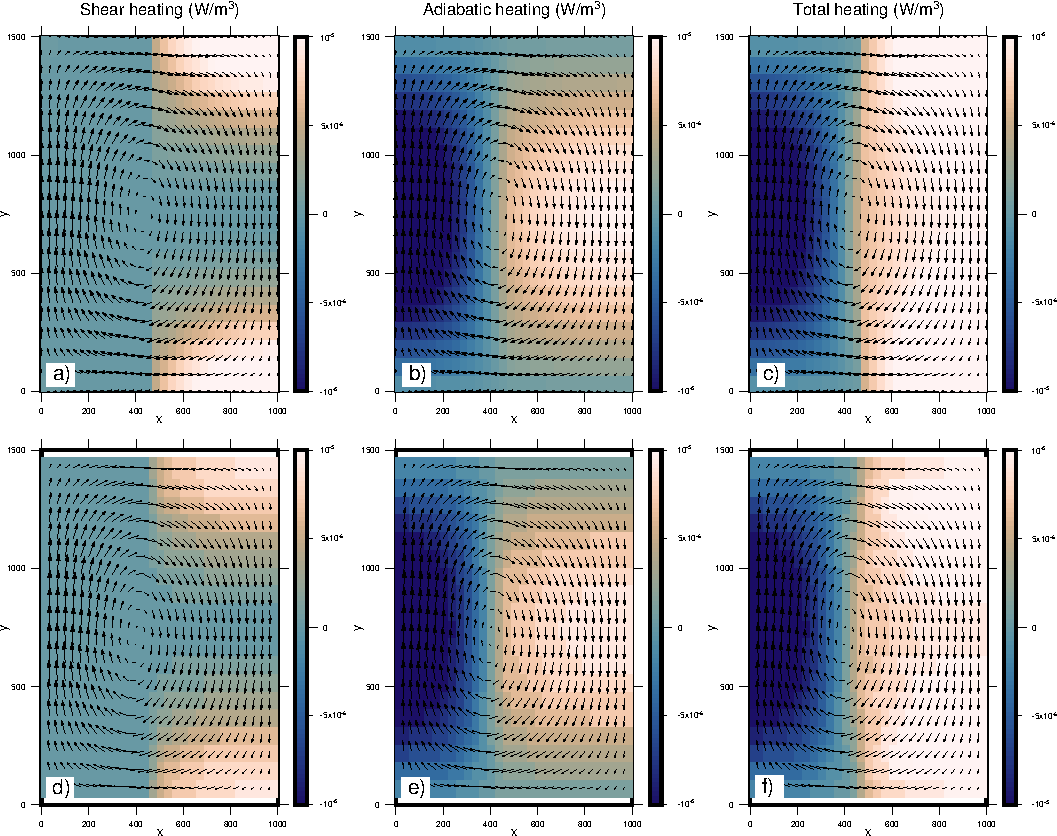
\includegraphics[width=400px]{./Figures/Energy.pdf}
\caption{Comparison between shear (first column), adiabatic (second column) and total (third column) energy predicted by the code (panels a, b and c) and those
created using example ${Shear\_adiabatic\_heating.m}$ from Exercise 9.4 in \citet{Gerya2010b} (panels d, e and f).}
\label{fig:energy}
\end{figure}

\subsection{Mantle convection}\label{sec:mantle}
This problem is performed as presented by \citet{Blankenbach1989} (constant viscosity cases) and \citet{Thieulot2014}, in a 2D unit square domain with gravity
acceleration $g_y=10^{10}Ra$. The experiment is performed with three different Rayleigh numbers ($Ra=10^4$, $10^5$ and $10^6$) and with different grid
resolution (between \num{32x32} and \num{128x128} elements). The fluid has constant viscosity, initial density, heat capacity, thermal conductivity
($\eta= \rho_0= C_p = k=1$), reference temperature ($T_0=0$) and thermal expansion coefficient ($\alpha=10^{-10}$). Temperatures are set to 0 on top and 1 on
bottom of the domain. Velocity boundary conditions are set to free slip on all sides. The initial temperature field is given by
\[T(x,y)=(1-y)+0.01 \cos (\pi x) \sin (\pi y)\]

The solution generated by the code in terms of $v_{\textrm{rms}}$ (calculated as in Sec. \ref{sec:error}) and Nu as function of time are reported for all the
simulations in Fig. \ref{fig:mantle}. At the steady state, $v_{\textrm{rms}}$ and Nu of all simulations converge well toward the values from \citet{Blankenbach1989},
with lower errors for higher resolution grids (Table \ref{tab:mantle}). All data can be found at 
\url{https://github.com/aleregorda/Benchmarks/tree/main/Momentum%2BEnergy/Mantle_convection}.

\begin{figure}
\centering
\noindent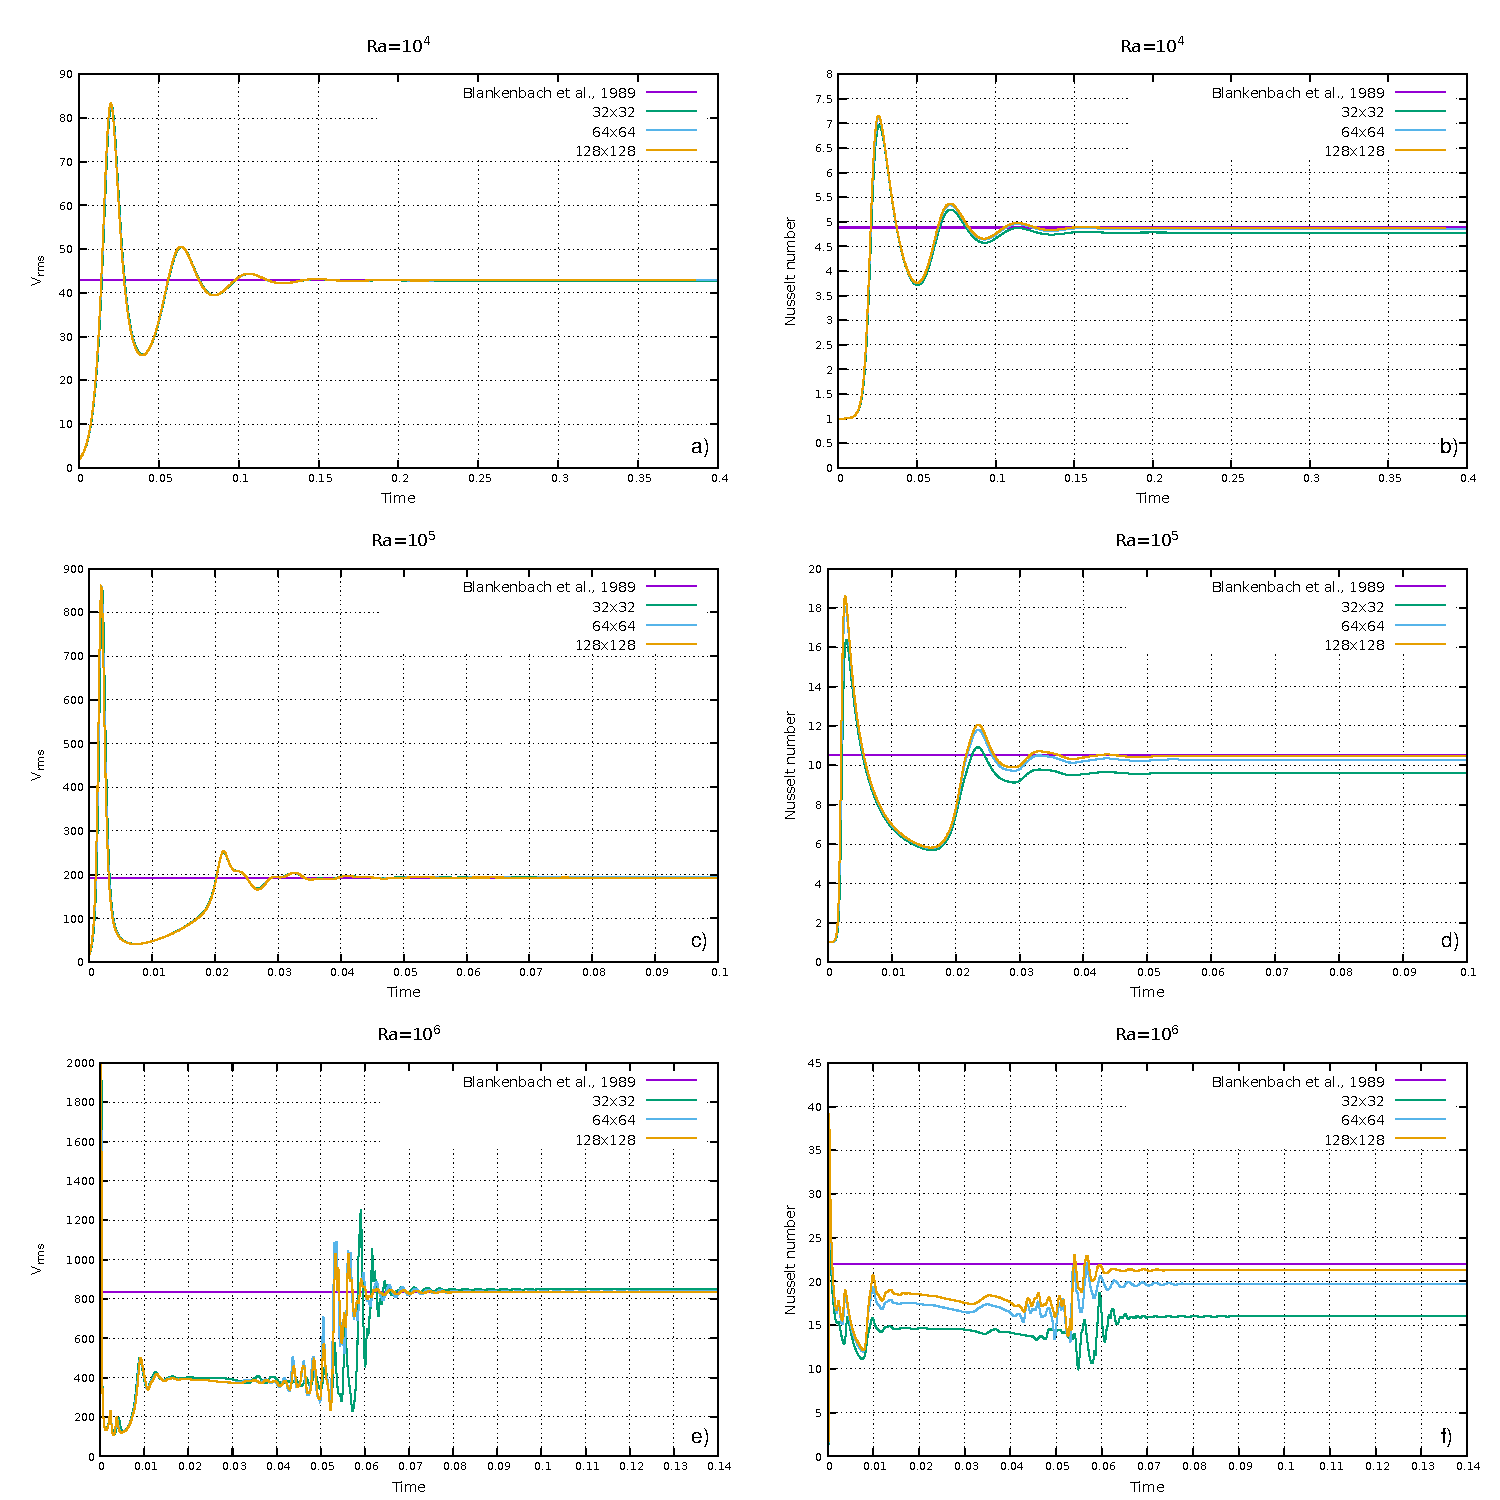
\includegraphics[width=400px]{./Figures/Convection.pdf}
\caption{$v_{\textrm{rms}}$ (panels a, c and e) and Nu (panels b, d and f) for the mantle convection benchmark as function of time for different grid resolution.
Panels a and b show the results for $Ra=10^4$; Panels c and d show the results for $Ra=10^5$; panels e and f show the results for $Ra=10^6$. Purple lines
indicate the convergence values for the $v_{\textrm{rms}}$ and the Nu from \citet{Blankenbach1989} at the steady state.}
\label{fig:mantle}
\end{figure}

\begin{table}[H]
\caption{Comparison between $v_{\textrm{rms}}$ and Nu predicted by the code for the mantle convection experiment and same values as reported in literature.}
\centering
\small
\begin{tabular}{|>{\centering}m{0.09\textwidth}|>{\centering}m{0.05\textwidth}|>{\centering}m{0.24\textwidth}|>{\centering}m{0.15\textwidth}|
  >{\centering}m{0.1\textwidth} >{\centering}m{0.1\textwidth} >{\centering\arraybackslash}m{0.1\textwidth}|}
\toprule
& & \multirow{2}{*}{\citet{Blankenbach1989}} & \citet{Thieulot2014} & \multicolumn{3}{c|}{FALCON}  \\
 & & & \num{200x200} & \num{32x32} & \num{64x64} & \num{128x128}  \\
\midrule
\multirow{2}{*}{$Ra=10^4$} & $v_{\textrm{rms}}$ & $42.864947 \pm 0.000020$ & 42.867 & 42.83226 & 42.852793 & 42.861394  \\
           & Nu      & $4.884409 \pm 0.000010$  & 4.882  & 4.781297 & 4.857475  & 4.877573   \\
\hline
\multirow{2}{*}{$Ra=10^5$} & $v_{\textrm{rms}}$ & $193.21454 \pm 0.00010$  & 193.255& 193.872643 & 193.377472 & 193.252290  \\
           & Nu      & $10.534095 \pm 0.000010$ & 10.507 & 9.602514 & 10.270735  & 10.465629   \\
\hline
\multirow{2}{*}{$Ra=10^6$} & $v_{\textrm{rms}}$ & $833.98977 \pm 0.00020$  & 834.712& 848.091176 & 837.767911 & 834.945793  \\
           & Nu      & $21.972465 \pm 0.000020$ & 21.695 & 15.999266 & 19.703682  & 21.306939   \\
\bottomrule
\end{tabular}
\label{tab:mantle}
\end{table}

\subsection{Viscoplastic mantle convection}\label{sec:visco_mantle}
This benchmark is performed as Cases 1-5a described in \citet{Tosi2015} in a 2D unit square domain with two different grid resolutions of \num{32x32} 
and \num{100x100} elements. Reference viscosity, reference density, heat capacity, thermal conductivity and thermal expansion coefficient are fixed to a constant
value of 1 ($\eta_0= \rho_0= C_p = k=\alpha=1$), while the gravity has been chosen as $g_y=10^2$, in order to obtain a Rayleigh number $Ra=10^2$. Temperatures
are set to 0 on top and 1 on bottom of the domain. Velocity boundary conditions are set to free slip on all sides. The initial temperature field is given by
\[T(x,y)=(1-y)+0.01 \cos (\pi x) \sin (\pi y)\].
The viscosity field $\eta$ is calculated as the harmonic average between a linear part $\eta_{lin}$ that depends on temperature only or on temperature and 
depth $y$ and a nonlinear-plastic part $\eta_{pl}$ that depends on the strain rate $\dot{\bm{\epsilon}}$, as follows
\[\eta(T,y,\dot{\bm{\epsilon}})=2\left(\frac{1}{\eta_{lin}(T,y)}+\frac{1}{\eta_{pl}(\dot{\bm{\epsilon}})}\right)^{-1}\]
The linear and the nonlinear-plastic parts of the viscosity are calculated following \citet{Tosi2015} as follows
\[\eta_{lin}(T,y)=\exp(-\ln(\Delta\eta_T)T+\ln(\Delta\eta_y)y)\]
\[\eta_{pl}(\dot{\bm{\epsilon}})=\eta^*+\frac{\sigma_Y}{\sqrt{\dot{\bm{\epsilon}}:\dot{\bm{\epsilon}}}}\]
where $\Delta\eta_T$, $\Delta\eta_y$, $\eta^*$ and $\sigma_Y$ are parameters chosen as listed in Table \ref{tab:tosi_setup}.

For each case, some diagnostic quantities measured at the steady state are reported in Table \ref{tab:visco_mantle} (see Section \ref{sec:error} for 
the computation of all the quantities), showing a well fit with results described in \citet{Tosi2015}. Data and charts for all cases can be found at 
\url{https://github.com/aleregorda/Benchmarks/tree/main/Momentum%2BEnergy/Viscoplastic_mantle_convection}.

%\renewcommand{\arraystretch}{1.5}
%{\rowcolors{3}{white!100!}{gray!25!}
%\begin{table}[H]
%  \caption{Results of the viscoplastic mantle convection benchmark for Cases 1-4 compared with results obtained with ELEFANT and YACC (from \citealp{Tosi2015}).}
%  \centering
%  \resizebox{\textwidth}{!}{
%\begin{tabular}{|c|ccc|ccc|ccc|ccc|}
%  \toprule
%    & \multicolumn{3}{c|}{\textbf{Case 1}} & \multicolumn{3}{c|}{\textbf{Case 2}} & \multicolumn{3}{c|}{\textbf{Case 3}} &
%    \multicolumn{3}{c|}{\textbf{Case 4}} \\
%   & FALCON & ELEFANT& YACC & FALCON& ELEFANT& YACC & FALCON & ELEFANT & YACC & FALCON & ELEFANT & YACC \\
%  \midrule
%   $\left\langle T \right\rangle$ & 0.7759 & 0.7758 & 0.7767 & 0.6043 & 0.6036 & 0.6058 & 0.7275 & 0.7275 & 0.7286 & & 0.5277 & 0.5289\\
%    Nu$^{top}$ & 3.4280 & 3.4214 & 3.4298 & 8.5242 & 8.5115 & 8.5278 & 3.0368 & 3.0347 & 3.0374 && 6.5912 & 6.5572 \\
%    Nu$^{bottom}$ & 3.3168 & 3.313 & 3.3143 & 8.4599 & 8.4465 & 8.3990 & 3.0086 & 2.9908 & 2.9628 && 6.5834 & 6.5243 \\
%    $v_{\textrm{rms}}$ & 249.901 & 249.134 & 251.7997 & 141.2451 & 140.7087 & 142.2020 & 100.2776 & 100.1208 & 100.9467 && 79.1105 & 79.6202 \\
%    $v_{\textrm{rms}}^{top}$ & 1.8907 & 1.8642 & 1.8298 & 104.7928 & 104.1228 & 105.1767 & 2.0832 & 2.0652 & 2.0374 && 74.7596 & 75.8414 \\
%    $u_{max}^{top}$ & 2.6340 & 2.6119 & 2.5516 & 121.9212& 121.766 & 122.3238 & 2.9086 & 2.9019 & 2.8458 && 88.9146 & 89.2940 \\
%    $\eta_{min}$ & - & - & - & $2.0303\times10^{-5}$ & $2.0600\times10^{-5}$ & $1.9853\times10^{-5}$ & $4.8129\times10^{-5}$ & $4.8080\times10^{-5}$ & $4.7907\times10^{-5}$ &
%    & $1.9860\times10^{-4}$ & $1.9174\times10^{-4}$ \\
%    $\eta_{max}$ & - & - & - & 1.3325 & 1.85 & 1.6095 & 0.9360 & 0.9023 & 1 && 1.52 & 1.6773 \\
%    $\left\langle W \right\rangle$ & 2.4299 & 2.4316 & 2.4583 & 7.5648 & 7.5665 & 7.6222 & 2.0387 & 2.0384 & 2.0400 && 5.6216 & 5.6512 \\
%    $\left\langle \Phi \right\rangle/Ra$ & 2.4311 & 2.4276 & 2.4333 & 7.5661 & 7.5585 & 7.6194 & 2.0386 & 2.0370 & 2.0335 && 5.6182 & 5.6463 \\
%    $\delta$ & 0.05\% & 0.16\% & 1.02\% & 0.02\% & 0.11\% & 0.04\% & $<$0.01\% & 0.07\% & 0.32\% && 0.06\% & 0.09\% \\
%  \bottomrule
%  \end{tabular}}
%  \label{tab:visco_mantle}
%  \end{table}
%\renewcommand{\arraystretch}{1.5}
%{\rowcolors{2}{white!100!}{gray!25!}
\begin{table}[H]
  \caption{Benchmark cases and corresponding parameters.}
  \centering
  \small
\begin{tabular}{|>{\centering}m{0.08\textwidth}|>{\centering}m{0.05\textwidth}>{\centering}m{0.05\textwidth}>{\centering}m{0.05\textwidth}
  >{\centering}m{0.05\textwidth} >{\centering}m{0.05\textwidth} |>{\centering\arraybackslash}m{0.2\textwidth}|}
  \toprule
    Case & $Ra$ & $\Delta\eta_T$ & $\Delta\eta_y$ & $\eta^*$ & $\sigma_Y$ & Convective regime \\
  \midrule
  \rowcolor{gray!25!}
    1 & $10^2$ & $10^5$ & 1 & - & - & Stagnant lid \\
    2 & $10^2$ & $10^5$ & 1 & $10^{-3}$ & 1 & Mobile lid  \\
    \rowcolor{gray!25!}
    3 & $10^2$ & $10^5$ & 10 & - & - & Stagnant lid  \\
    4 & $10^2$ & $10^5$ & 10 & $10^{-3}$ & 1 & Mobile lid \\
    \rowcolor{gray!25!}
    5 & $10^2$ & $10^5$ & 10 & $10^{-3}$ & 4 & Periodic \\
  \bottomrule
  \end{tabular}
  \label{tab:tosi_setup}
  \end{table}

\renewcommand{\arraystretch}{1.5}
%{\rowcolors{3}{gray!25!}{white!100!}
\begin{table}
  \caption{Results of the viscoplastic mantle convection benchmark for different grid resolutions in Cases 1-5 compared with results obtained with ELEFANT
  and YACC ($100\times100$ elements, from \citealp{Tosi2015}) and in Stone 28 ($32\times32$ elements, from
  \url{https://github.com/cedrict/fieldstone/tree/master/python_codes/fieldstone_28}).}
  \centering
  \resizebox{\textwidth}{!}{
\begin{tabular}{|cc|ccccccccccc|}
  \toprule
  \multicolumn{13}{|c|}{\textbf{Case 1}} \\
  \midrule
  Code & Resolution & $\left\langle T \right\rangle$ & Nu$^{top}$ & Nu$^{bottom}$ & $v_{\textrm{rms}}$ & $v_{\textrm{rms}}^{top}$& $u_{max}^{top}$& $\eta_{min}$
  & $\eta_{max}$ & $\left\langle W \right\rangle$ & $\left\langle \Phi \right\rangle/Ra$ & $\delta$ \\
  \hline
  \rowcolor{gray!25!}
    YACC & $100\times100$ & 0.7767 & 3.4298 & 3.3143 & 251.7997 & 1.8298 & 2.5516 & - & - & 2.4583 & 2.4333 & 1.02\% \\
    ELEFANT & $100\times100$ & 0.7758 & 3.4214 & 3.313 & 249.134 & 1.8642 & 2.6119 & - & - & 2.4316 & 2.4276 & 0.16\% \\
    \rowcolor{gray!25!}
    Stone 28 & $32\times32$ & 0.7737 & 3.3987 & - & 243.872 & - & - & - & - & - & - & - \\
%    FALCON & $32\times32$ & 0.7750 & 3.4381 & 2.7363 & 248.3337 & 2.0022 & 2.7813 & - & - & 2.4745 & 2.4864 & 0.48\% \\
%    \rowcolor{gray!25!}
    FALCON & $100\times100$ & 0.7759 & 3.4280 & 3.3168 & 249.901 & 1.8907 & 2.6340 & - & - & 2.4299 & 2.4311 & 0.05\% \\
    \midrule
    \multicolumn{13}{|c|}{\textbf{Case 2}} \\
    \midrule
    Code & Resolution & $\left\langle T \right\rangle$ & Nu$^{top}$ & Nu$^{bottom}$ & $v_{\textrm{rms}}$ & $v_{\textrm{rms}}^{top}$& $u_{max}^{top}$& $\eta_{min}$
    & $\eta_{max}$ & $\left\langle W \right\rangle$ & $\left\langle \Phi \right\rangle/Ra$ & $\delta$ \\
    \hline
    \rowcolor{gray!25!}
     YACC & $100\times100$ & 0.6058 & 8.5278 & 8.3990 & 142.2020 & 105.1767 & 122.3238 & $1.9853\times10^{-5}$ & 1.6095 & 7.6222 & 7.6194 & 0.04\% \\
     ELEFANT & $100\times100$ & 0.6034 & 8.5115 & 8.4465 & 140.8067 & 104.1228 & 121.766 & $2.0600\times10^{-5}$ & 1.85 & 7.5665 & 7.5585 & 0.11\% \\
     \rowcolor{gray!25!}
     Stone 28 & $32\times32$ & 0.6052 & 8.1715 & - & 141.518 & - & - & - & - & - & - & - \\
%     FALCON & $32\times32$ & 0.6454 & 8.1422 & 7.4020 & 156.6908 & 95.7226 & 116.9302 & $2.2572\times10^{-5}$ & 0.7194 & 7.4289 & 7.4452 & 0.22\% \\
%     \rowcolor{gray!25!}
     FALCON & $100\times100$ & 0.6044 & 8.5266 & 8.4590 & 141.3684 & 104.8867 & 122.0470 & $2.0333\times10^{-5}$ & 1.2914 & 7.5707 & 7.5718 & 0.01\% \\
     \midrule
     \multicolumn{13}{|c|}{\textbf{Case 3}} \\
     \midrule
     Code & Resolution & $\left\langle T \right\rangle$ & Nu$^{top}$ & Nu$^{bottom}$ & $v_{\textrm{rms}}$ & $v_{\textrm{rms}}^{top}$& $u_{max}^{top}$& $\eta_{min}$
     & $\eta_{max}$ & $\left\langle W \right\rangle$ & $\left\langle \Phi \right\rangle/Ra$ & $\delta$ \\
     \hline
     \rowcolor{gray!25!} 
     YACC & $100\times100$ & 0.7286 & 3.0374 & 2.9628 & 100.9467 & 2.0374 & 2.8458 & $4.7907\times10^{-5}$ & 1 & 2.0400 & 2.0335 & 0.32\% \\
      ELEFANT & $100\times100$ & 0.7275 & 3.0347 & 2.9908 & 100.1208 & 2.0652 & 2.9019 & $4.8080\times10^{-5}$ & 0.9023 & 2.0384 & 2.037 & 0.07\% \\
      \rowcolor{gray!25!}
      Stone 28 & $32\times32$ & 0.7277 & 3.0347 & - & 100.018 & - & - & - & - & - & - & - \\
%      FALCON & $32\times32$ & 0.7281 & 3.0618 & 2.8132 & 101.0092 & 2.1630 & 3.0178 & $4.8500\times10^{-5}$ & 0.7845 & 2.0699 & 2.0695 & 0.02\% \\
%      \rowcolor{gray!25!}
      FALCON & $100\times100$ & 0.7275 & 3.0368 & 3.0086 & 100.2776 & 2.0832 & 2.9086 & $4.8129\times10^{-5}$ & 0.9360 & 2.0387 & 2.0386 & $<$0.01\% \\
      \midrule
      \multicolumn{13}{|c|}{\textbf{Case 4}} \\
      \midrule
      Code & Resolution & $\left\langle T \right\rangle$ & Nu$^{top}$ & Nu$^{bottom}$ & $v_{\textrm{rms}}$ & $v_{\textrm{rms}}^{top}$& $u_{max}^{top}$& $\eta_{min}$
      & $\eta_{max}$ & $\left\langle W \right\rangle$ & $\left\langle \Phi \right\rangle/Ra$ & $\delta$ \\
      \hline
      \rowcolor{gray!25!} 
      YACC & $100\times100$ & 0.5289 & 6.5572 & 6.5243 & 79.6202 & 75.4814 & 89.2940 & $1.9174\times10^{-4}$ & 1.6773 & 5.6512 & 5.6463 & 0.09\% \\
       ELEFANT & $100\times100$ & 0.5277 & 6.5912 & 6.5834 & 79.1105 & 74.7596 & 88.9146 & $1.9860\times10^{-4}$ & 1.5200 & 5.6216 & 5.6182 & 0.06\% \\
       \rowcolor{gray!25!}
       Stone 28 & $32\times32$ & 0.5286 & 6.4036 & - & 79.4746 & - & - & - & - & - & - & - \\
%       FALCON & $32\times32$ & 0.5334 & 6.4679 & 6.3435 & 80.6153 & 76.0511 & 90.2058 & $2.0393\times10^{-4}$ & 0.6453 & 5.6676 & 5.6698 & 0.04\% \\
%       \rowcolor{gray!25!}
       FALCON & $100\times100$ & 0.5279 & 6.5897 & 6.5830 & 79.1220 & 75.0715 & 88.8484 & $1.9693\times10^{-4}$ & 1.4133 & 5.6127 & 5.6113 & 0.03\% \\
       \midrule
       \multicolumn{13}{|c|}{\textbf{Case 5}} \\
       \midrule
       Code & Resolution & $P$ & $\left\langle T \right\rangle_{min}$ & $\left\langle T \right\rangle_{max}$ & Nu$^{top}_{min}$ & Nu$^{top}_{max}$ &
       $v_{\textrm{rms}}^{min}$ & $v_{\textrm{rms}}^{max}$ & \multicolumn{2}{c}{$(\left\langle \Phi \right\rangle/Ra)_{min}$} & 
       \multicolumn{2}{c|}{$(\left\langle \Phi \right\rangle/Ra)_{max}$} \\
       \hline
       \rowcolor{gray!25!}
         YACC & $100\times100$ & 0.0792 & 0.6543 & 0.6722 & 2.6950 & 7.2792 & 41.9813 & 98.8230 & \multicolumn{2}{c}{1.4347} & 
         \multicolumn{2}{c|}{9.2748} \\
         ELEFANT & $100\times100$ & 0.076 & 0.6514 & 0.6693 & 2.6808 & 7.3506 & 41.2578 & 100.089 & \multicolumn{2}{c}{1.3324} & 
         \multicolumn{2}{c|}{9.5289} \\
         \rowcolor{gray!25!}
         Stone 28 & $32\times32$ & 0.0764 & 0.6521 & 0.6697 & 2.6912 & 7.0763 & 41.61 & 98.183 & \multicolumn{2}{c}{-} & 
         \multicolumn{2}{c|}{-} \\
     %    FALCON & $32\times32$ & & 0.7750 & 3.4381 & 2.7363 & 248.3337 & 2.0022 & 2.7813 & \multicolumn{2}{c}{-} & 
     %     \multicolumn{2}{c|}{-} \\
     %    \rowcolor{gray!25!}
         FALCON & $100\times100$ & 0.0775 & 0.6519 & 0.6697 & 2.6847 & 7.3629 & 41.5256 & 99.5466 & \multicolumn{2}{c}{1.3399} & 
         \multicolumn{2}{c|}{9.3993} \\
  \bottomrule
  \end{tabular}}
  \label{tab:visco_mantle}
  \end{table}

\subsection{Thin layer entrainment}\label{sec:thin}
This experiment is performed as originally proposed by \citet{vanKeken1997} with two incompressible fluids in a rectangular domain with $L_x=2$ and $L_y=1$
and gravity acceleration $g_y=10^{10}Ra$. The Rayleigh number and the compositional Rayleigh number are fixed to $Ra=300000$ and $Rc=450000$, respectively.
Both fluids have constant viscosity, thermal conductivity, specific heat ($\eta=\rho=C_p=1$) and thermal expansion coefficient ($\alpha=10^{-10}$). Fluid 1
has a density $\rho_1=1$, while fluid 2 is denser ($\rho_2=\rho_1+1.5 \cdot 10^{-10}$) and is placed at the bottom of the domain, for $y \leq 0.025$.
Temperature are set to 0 on top and 1 on bottom of the domain. Velocity boundary conditions are set to free slip on all sides of the domain. The initial
temperature field is given by
\[T(x,y)=T_u(x,y)+T_l(x,y)+T_r(x,y)+T_s(x,y)-\frac{3}{2}\]
with
\begin{eqnarray}
T_u(x,y)&=&\frac{1}{2}erf\left(\frac{1-y}{2}\sqrt{\frac{u_0}{x}}\right)\nonumber \\
T_l(x,y)&=&1-\frac{1}{2}erf\left(\frac{y}{2}\sqrt{\frac{u_0}{L_x-x}}\right)\nonumber \\
T_r(x,y)&=&\frac{1}{2}+\frac{Q}{2\sqrt{\pi}}\sqrt{\frac{u_0}{y+1}} \exp\left(-\frac{x^2u_0}{4y+4}\right)\nonumber \\
T_s(x,y)&=&\frac{1}{2}-\frac{Q}{2\sqrt{\pi}}\sqrt{\frac{u_0}{2-y}} \exp\left(-\frac{(L_x-x)^2u_0}{8-4y}\right)\nonumber
\end{eqnarray}
and
\begin{eqnarray}
u_0&=&\frac{L_x^{7/3}}{(1+L_x^4)^{2/3}}\left(\frac{Ra}{2\sqrt{\pi}}\right)^{\frac{2}{3}}\nonumber \\
Q&=&2\sqrt{\frac{L_x}{\pi u_0}}\nonumber
\end{eqnarray}

The experiment is performed with two grid resolution (\num{125x40} and \num{200x80} elements), with 100 markers per element and CFL of 0.25. $v_{\textrm{rms}}$
(see Sec. \ref{sec:error}) calculated for both the simulations match well with results from \citet{vanKeken1997} and obtained with ASPECT
\citep{KHB12,heister_aspect_methods2,aspect-doi-v2.2.0,aspectmanual} and ELEFANT \citep{Thieulot2014}, obtained with similar grid resolutions
(Fig. \ref{fig:thin}). In addition, a variety of simulations with different resolutions and aspect ratios are performed to verify that the sensitivity of the
initial velocity field. Results match well with results from \citet{vanKeken1997} (in the grey area) and \citet{Thieulot2014} (Fig. \ref{fig:thin_initial}). 
All data can be found at \url{https://github.com/aleregorda/Benchmarks/tree/main/Momentum%2BEnergy/Thin_layer}.

\begin{figure}
\centering
\noindent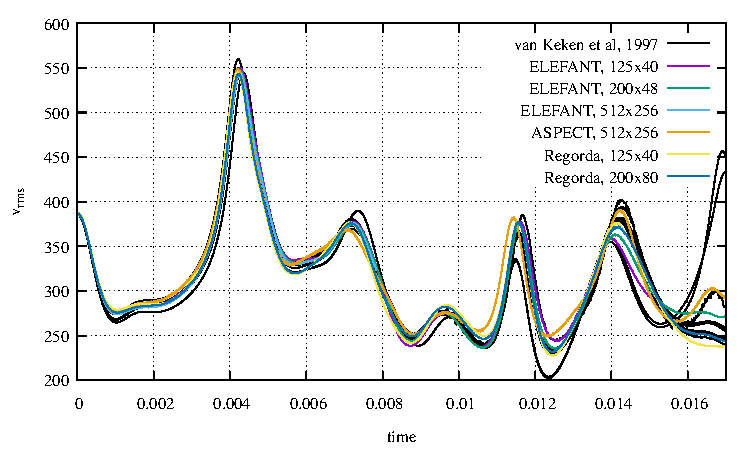
\includegraphics[width=400px]{./Figures/vrms_thin.pdf}
\caption{$v_{\textrm{rms}}$ for the thin layer experiment as function of time for different grid resolution. Results are compared with results obtained by
\citet{vanKeken1997} (black lines) and with ASPECT and ELEFANT.}
\label{fig:thin}
\end{figure}

\begin{figure}
\centering
\noindent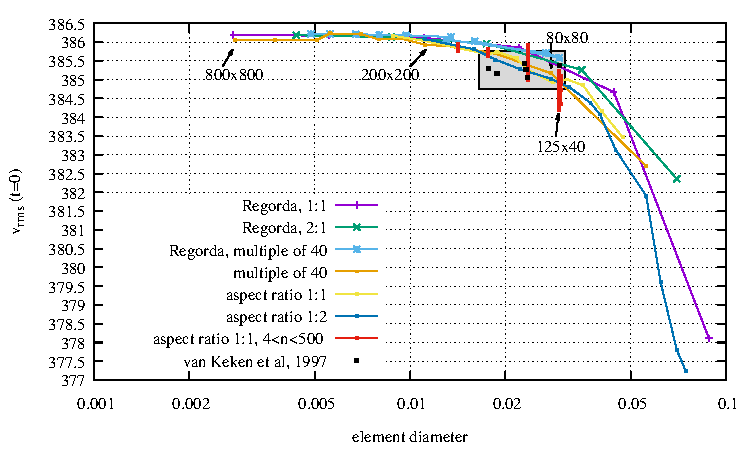
\includegraphics[width=400px]{./Figures/vrmszero.pdf}
\caption{$v_{\textrm{rms}}$ at $t=0$ for the thin layer experiment as function of the element size for different aspect ratios of the elements. Results are compared
with results obtained by \citet{vanKeken1997} (black dots in the grey area) and with ASPECT and ELEFANT.}
\label{fig:thin_initial}
\end{figure}

\subsection{Sinking hydrated cylinder}\label{sec:quinquis}
This experiment is performed as explained in \citet{Quinquis2014} and simulates the sinking of a cold, hydrated cylinder into a warm, dry mantle. The domain
is square with $L_x=L_y=$ \SI{300}{\km}, a grid resolution of \num{300x300} elements and 25 markers per element. The sinking cylinder is located at $x=$
\SI{150}{\km} and $y=$ \SI{170}{\km} with a radius of \SI{20}{\km} and has $\rho_c=$ \SI{3250}{\kg\per\cubic\m}, $\eta_c=$ \SI{e23}{\pascal\s}, a thermal
conductivity $k_c=$ \SI{4.5}{\watt\per\m\per\kelvin},a specific heat $C_{p_c}=$ \SI{1250}{\joule\per\kg\per\kelvin}; the surrounding mantle has $\rho_m=$
\SI{3200}{\kg\per\cubic\m}, $\eta_m=$ \SI{e20}{\pascal\s}, a thermal conductivity $k_m=$ \SI{105}{\watt\per\m\per\kelvin} and specific heat $C_{p_m}=$
\SI{1250}{\joule\per\kg\per\kelvin}; a 58 km-thick lithosphere overlies the mantle and has $\rho_l=$ \SI{3200}{\kg\per\cubic\m}, $\eta_l=$ \SI{e23}{\pascal\s},
a thermal conductivity $k_l=$ \SI{4.5}{\watt\per\m\per\kelvin}, specific heat $C_{p_l}=$ \SI{750}{\joule\per\kg\per\kelvin} and a thermal diffusivity of
\SI{e-6}{\square\m\per\s}. Velocity boundary conditions are set to free slip on all sides of the domain. Temperature increase linearly in the lithosphere,
from 0° to 1300°C, and in the mantle, from 1300° to 1360.5°C. The initial temperature of the cylinder is fixed to 400°C. Throughout the evolution, temperature
is fixed to 0° and 1360.5°C at the top and bottom of the domain, respectively. The initial bound water content is imposed at 2 wt.\% in the cylinder and at
0 wt.\% in both the mantle and the lithosphere. The maximum amount of water in the mantle is fixed to 0.2 wt.\%, while maximum water content in the cylinder
and in the lithosphere is function of pressure and temperature and is calculated using a serpentinized harzburgite with Perple\_X, as in \citet{Quinquis2014}.

As shown in \citet{Quinquis2014}, the model is characterised by a progressive dehydration in the external portion of the cylinder, due to the increase of
temperature, with a consequent vertical migration of free water that hydrates the mantle above the cylinder, up to the lithosphere. The distribution of
bound and free water during the evolution of the experiment is shown in Fig. \ref{fig:quinquis} (left and right columns, respectively). 
All data can be found at \url{https://github.com/aleregorda/Benchmarks/tree/main/Hydration}.

\begin{figure}
\centering
\noindent\includegraphics[width=400px]{./Figures/Hydration.pdf}
\caption{Distribution of bound and free water (left and right columns, respectively) at $t=0.5$ and $t=$ \SI{1.25}{\mega\year} (first and second rows,
respectively) for the sinking hydrated cylinder experiment. Only markers with bound or free water not equal to 0 are plotted.}
\label{fig:quinquis}
\end{figure}

\subsection{Mantle melting curves}\label{sec:katz}
This instantaneous experiment is performed in order to recreate isobaric melting curves, as function of temperature, bulk water and content of water in the
melt, to compare with melting curves obtained by \citet{Katz2003}. The domain is square with $L_x=L_y=100$ km, a grid resolution of \num{100x100} elements and
25 markers per element. Density is set in the entire domain to \SI{3300}{\kg\per\cubic\m} and temperature increases from the sides to the centre from 1000° to
1500°C. The experiment is performed for bulk water contents from 0 to 0.3 wt.\%.

Fig. \ref{fig:fraction} shows isobaric melting curves for \SI{1}{\giga\pascal} (panel a) and \SI{3}{\giga\pascal} (panel b) calculated for different bulk water
contents. The curves well match with those obtained for the mantle by \citet{Katz2003}, showing the saturation at the solidus for bulk water of 0.2 and 0.3 wt.\%, indicating
that the code correctly determines melt fraction as function of pressure, temperature and bulk water content. Same results can be observed in Fig.
\ref{fig:water}a, where isobaric and isothermal melting curves are shown as function of bulk water content. In addition, Fig. \ref{fig:water}b shows that the
code correctly determines also the percentage of water in the melt as function of pressure, temperature and melt fraction. 
All data can be found at \url{https://github.com/aleregorda/Benchmarks/tree/main/Melting}.

\begin{figure}
\noindent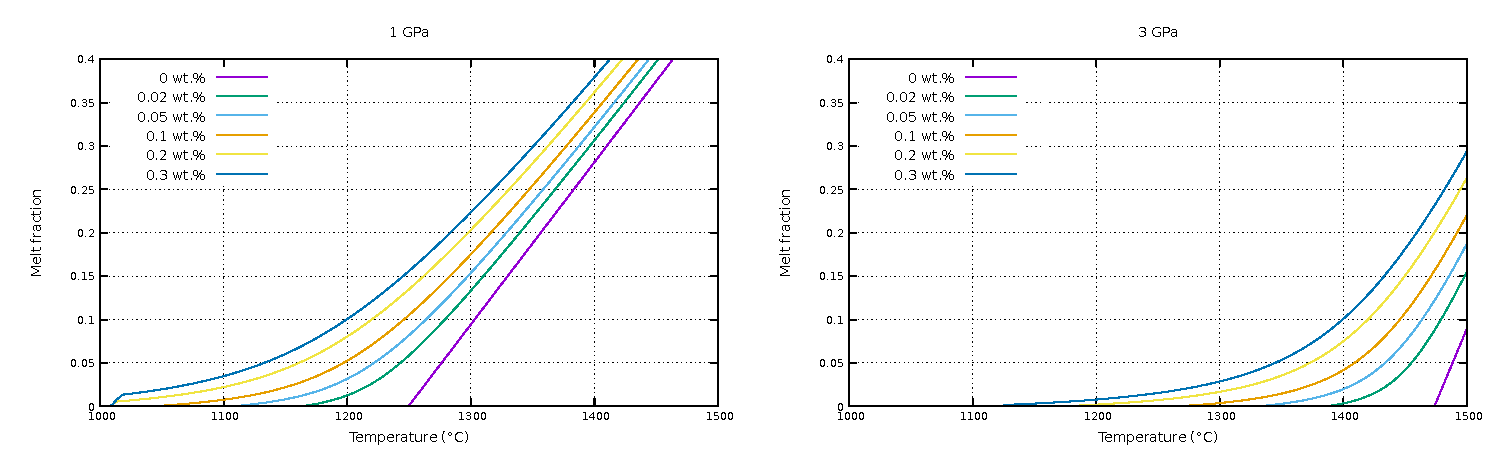
\includegraphics[width=\textwidth]{./Figures/Fraction.pdf}
\caption{Isobaric melting curves for 1 GPa (panel a) and 3 GPa (panel b) as function of temperature with different bulk water contents.}
\label{fig:fraction}
\end{figure}

\begin{figure}
\noindent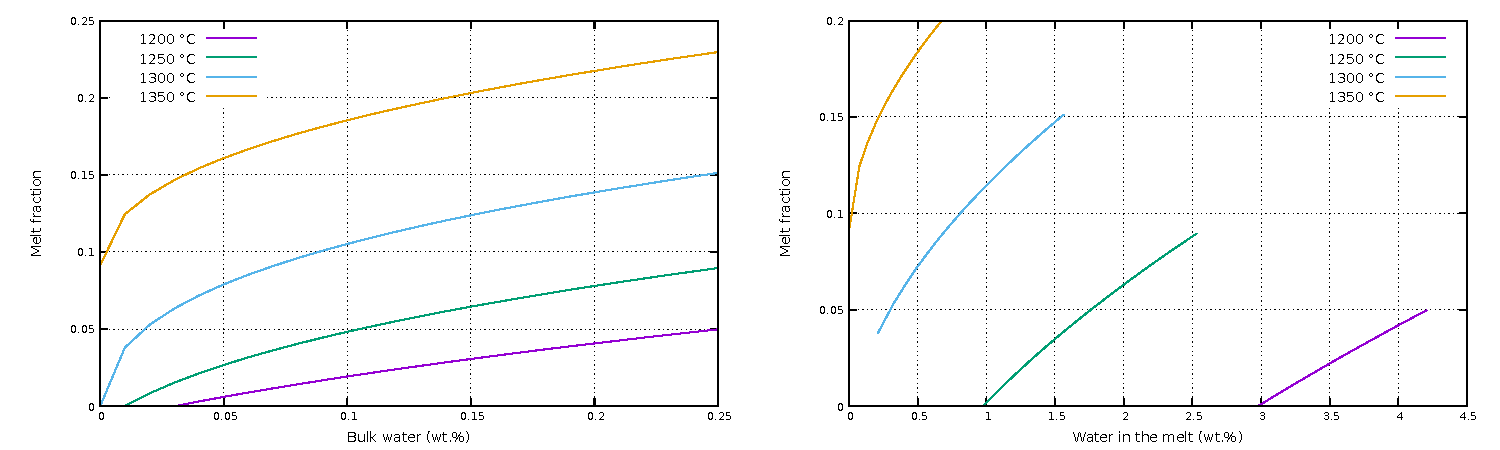
\includegraphics[width=\textwidth]{./Figures/Water.pdf}
\caption{Isobaric melting curves for 1.5 GPa as function of bulk water (panel a) and water in the melt (panel b) calculated for different temperatures.}
\label{fig:water}
\end{figure}

\clearpage

\bibliography{export}

\end{document}